\documentclass[12pt]{article}

\usepackage{amsmath}
\usepackage{amssymb}
\usepackage{amsfonts}
\usepackage[style=iso]{datetime2}
\usepackage[explicit]{titlesec}
\usepackage{amsthm}
\usepackage{array}
\usepackage{graphicx}
\usepackage{float}

\graphicspath{ {./Images/} }

\theoremstyle{definition}
\newtheorem{problem}{Problem}
\newtheorem{definition}{Definition}

\begin{titlepage}
\title{Calculus I: Review of Common Graphs}
\author{The Melon Man}
\date{\today}
\end{titlepage}

\renewcommand{\thesection}{\Roman{section}}

\allowdisplaybreaks

\setlength{\parindent}{0pt}
\setlength{\parskip}{1em}

\begin{document}
\maketitle

The purpose of this section is to be familiarised with the graphs of some the common functions found in a Calculus course.
We can use the graphs to analyse certain properties of the functions which may be helpful to us for certain problems.

\begin{problem}
Graph $\displaystyle f(x) = -\frac{2}{5}x + 3$.
\end{problem}

We know that this is a linear function, thus it describes a straight line.
It is in the form $y=mx+c$ where $m$ is the gradient and $c$ is the $y$-intercept (where the line crosses the $y$-axis).
We know that $(0, 3)$ will be one point on the line which is given to us by the $y$-intercept being 3.
i.e. when $x=0$ (the position of the $y$-axis), the value of $f(x)$ is 3.
We can find another point in the line by using some other $x$ value.
At $x=5$, $f(x)=1$ so we can use $(5, 1)$.

Since this function describes a straight line, only two points are needed as a line going through them will be the line described by $f(x)$.
The sketched function is then:

\begin{figure}[H]
    \centering
    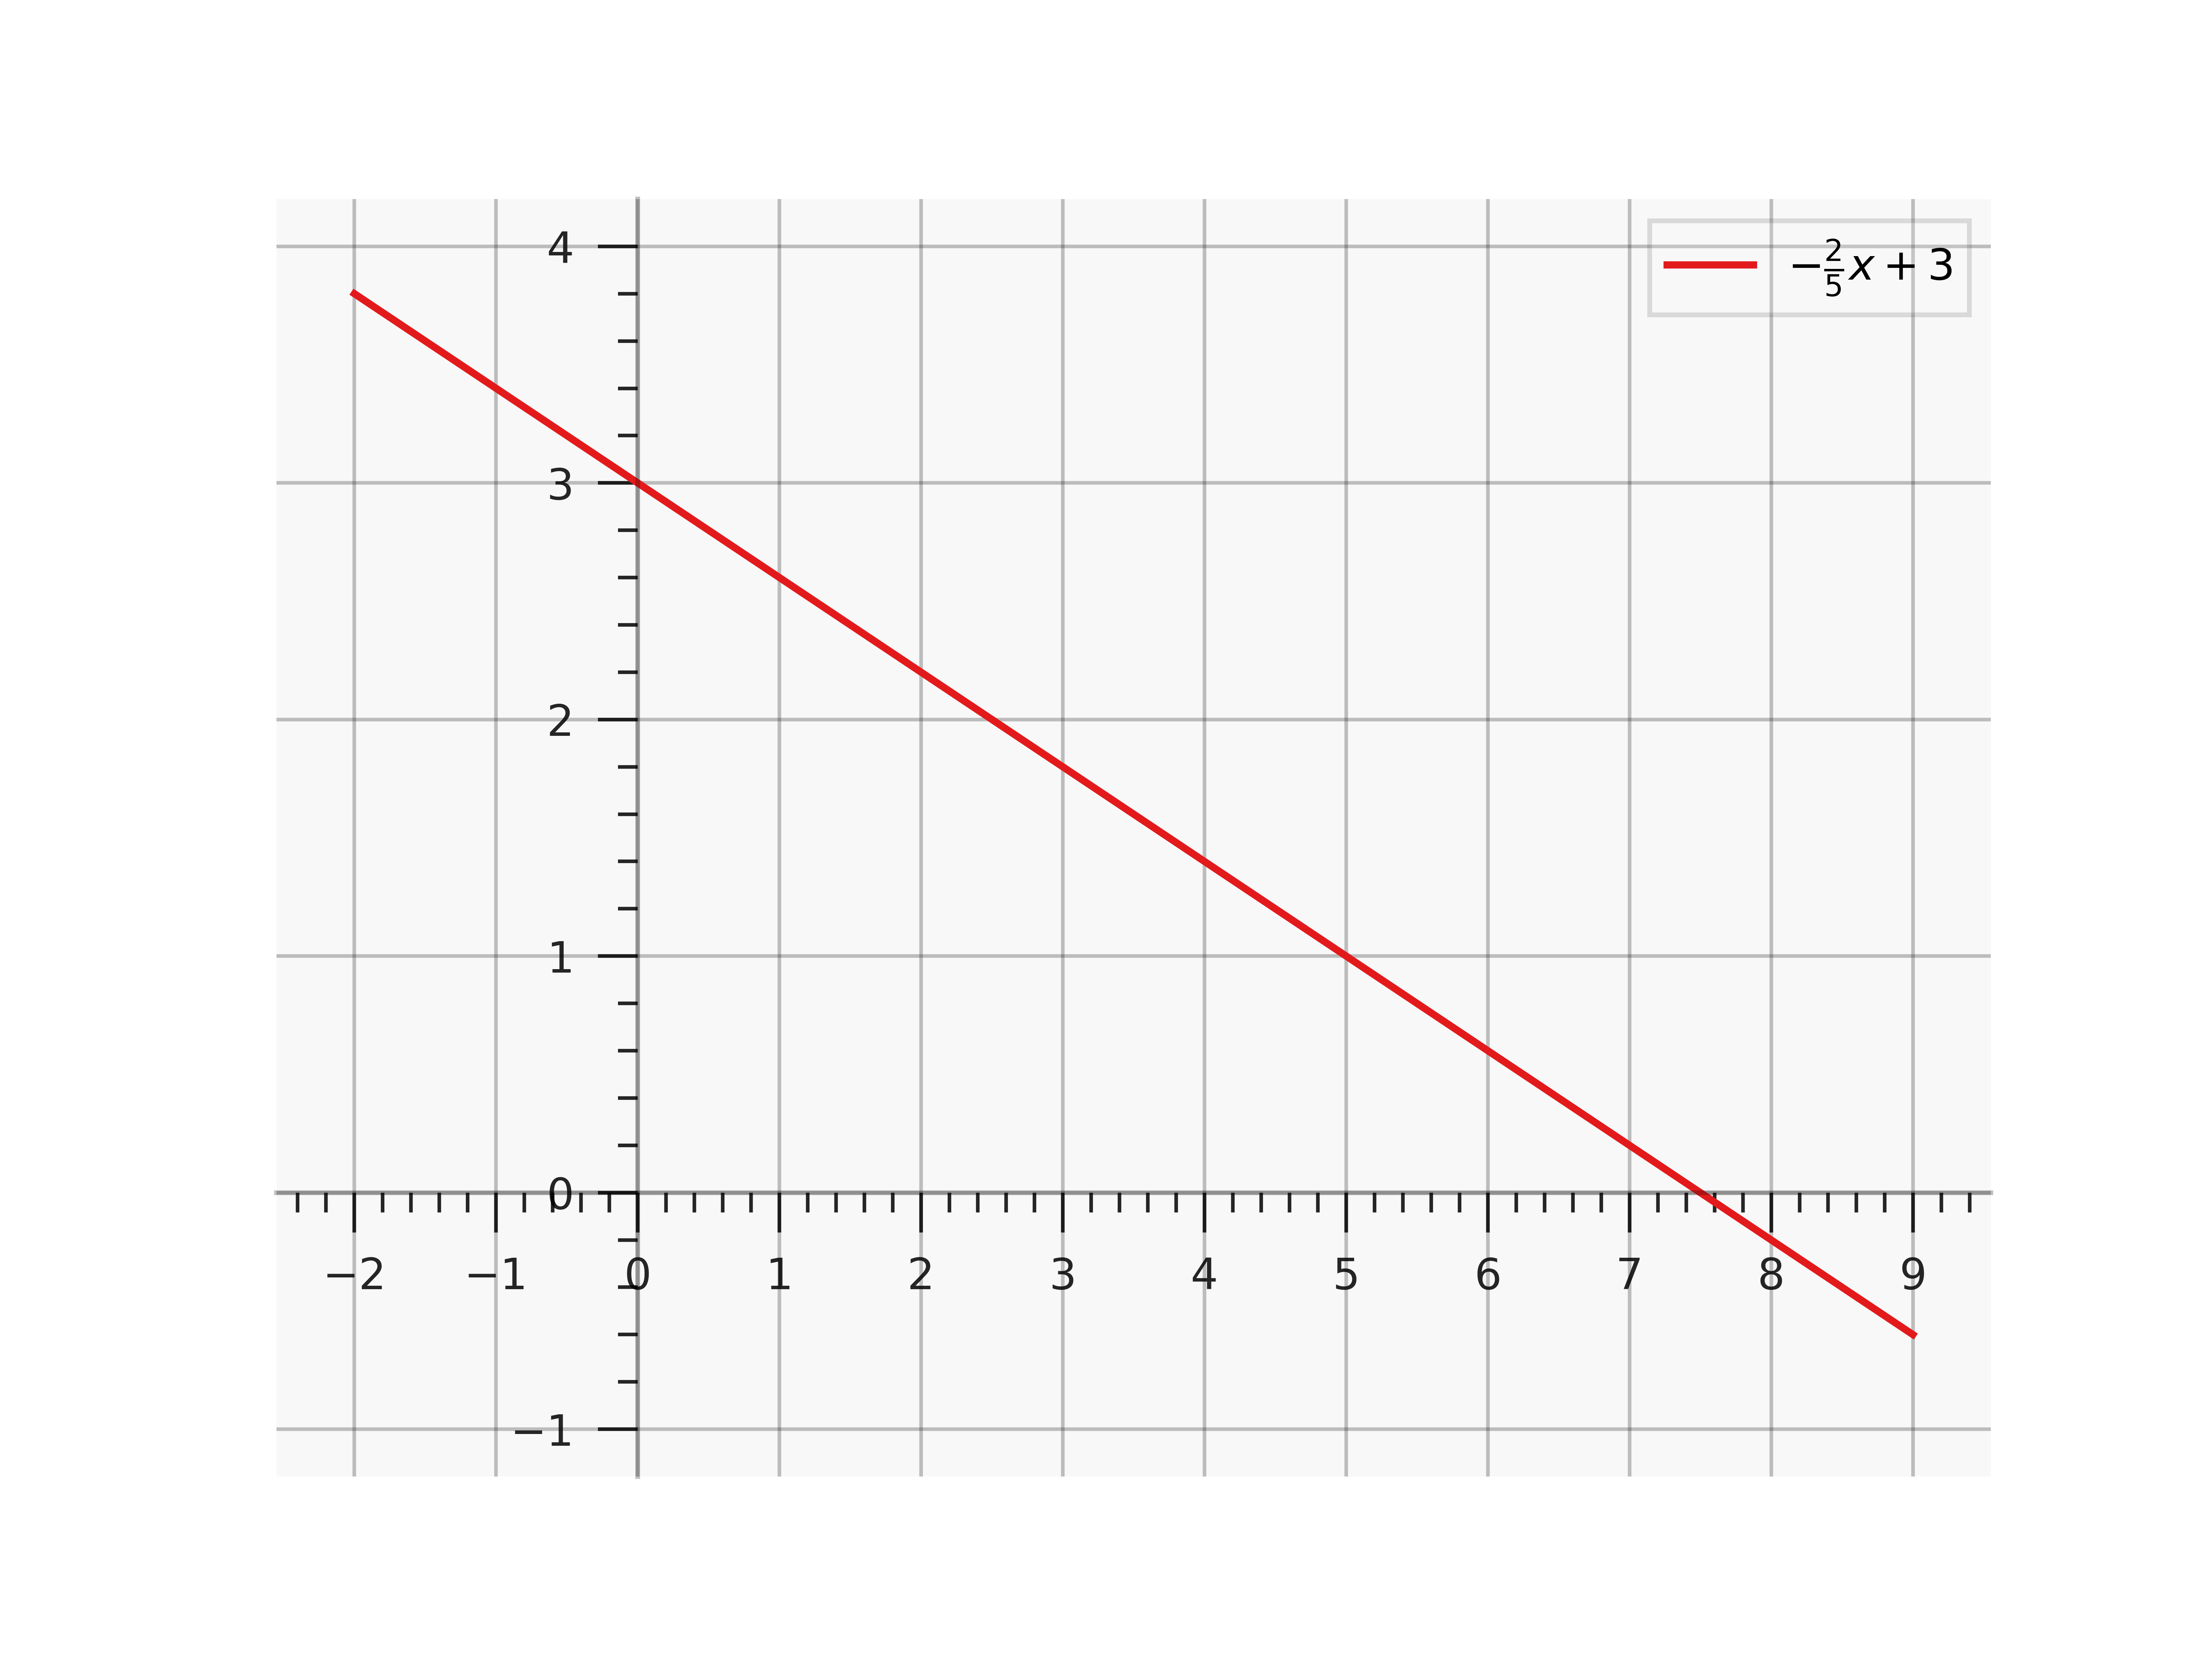
\includegraphics[width=10cm, keepaspectratio]{graph_1.png}
    \caption{Linear Functions}
    \label{fig:fig1}
\end{figure}

\begin{problem}
Graph $f(x) = |x|$.
\end{problem}

There isn't much too this besides remembering the definition of the absolute value function.
That is,

\begin{equation}
    |x| =
    \begin{cases}
        \phantom{-} x & \text{if } x \geq 0 \\
        -x            & \text{if } x < 0
    \end{cases}
\end{equation}

The graph would then be:

\begin{figure}[H]
    \centering
    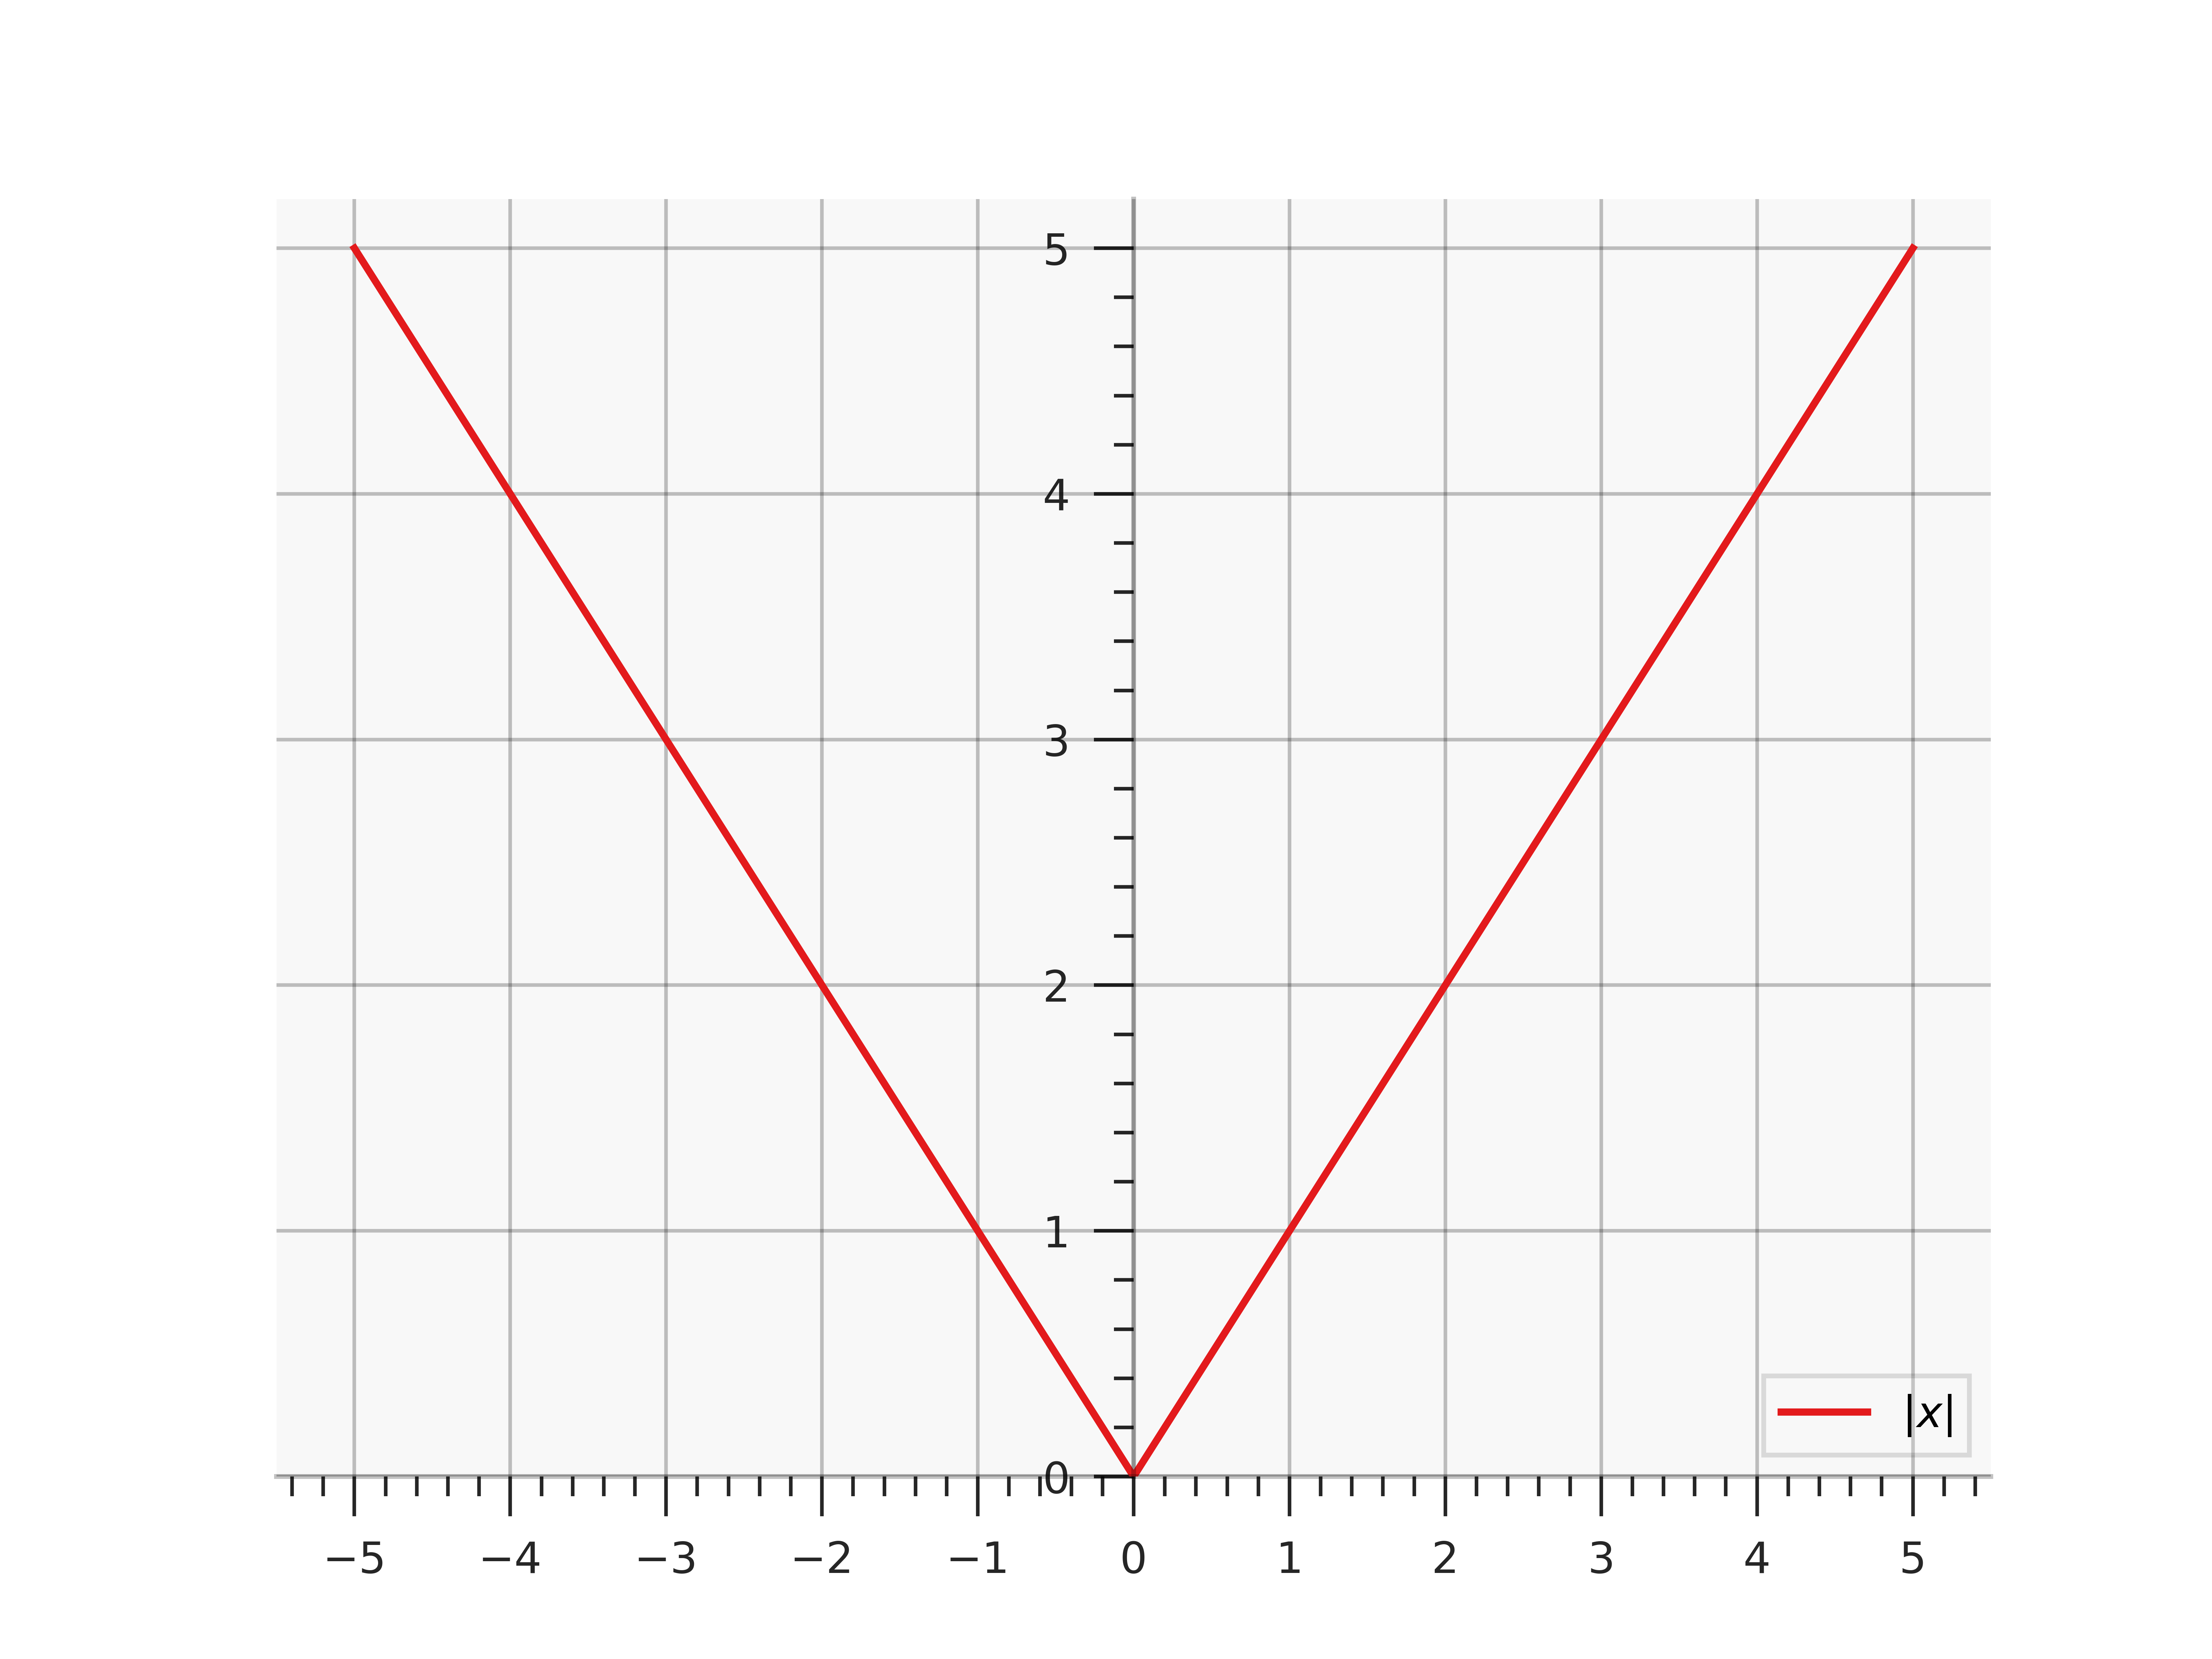
\includegraphics[width=10cm, keepaspectratio]{graph_2.png}
    \caption{Absolute Value Functions}
    \label{fig:fig2}
\end{figure}

\begin{problem}
Graph $f(x) = -x^2+2x+3$.
\end{problem}

This is a function of a quadratic polynomial in the standard form.

\begin{equation}
    f(x) = ax^2 + bx + c
\end{equation}

Here, $a=-1$, $b=2$, and $c=-3$.
With this form, we can find the vertex (the highest or lowest point) with $x=-\frac{b}{2a}$.
For this, that would be $-\frac{2}{2(-1)}$ which is 1.
The $y$-coordinate for this point would then be $f(1)$ which is 4.
We then know that the vertex is $(1, 4)$.

As $a$ is negative, we know that the parabola represented by the function opens down (like a rainbow).
One thing this tells us is that the vertex we found above is the highest point on the parabola.
As the vertex is above the $x$-axis and the parabola opens down, we know that it will have points where it intersects with the $x$-axis.
These points are where $f(x)=0$.

\begin{align}
    -x^2+2x+3  & = 0  \\
    x^2-2x-3   & = 0  \\
    (x-3)(x+1) & = 0  \\
    \nonumber         \\
    x          & = 3  \\
               & \&   \\
    x          & = -1
\end{align}

We multiplied everything by $-1$ to make factorising the equation easier.
Our sketch of the parabola is:

\begin{figure}[H]
    \centering
    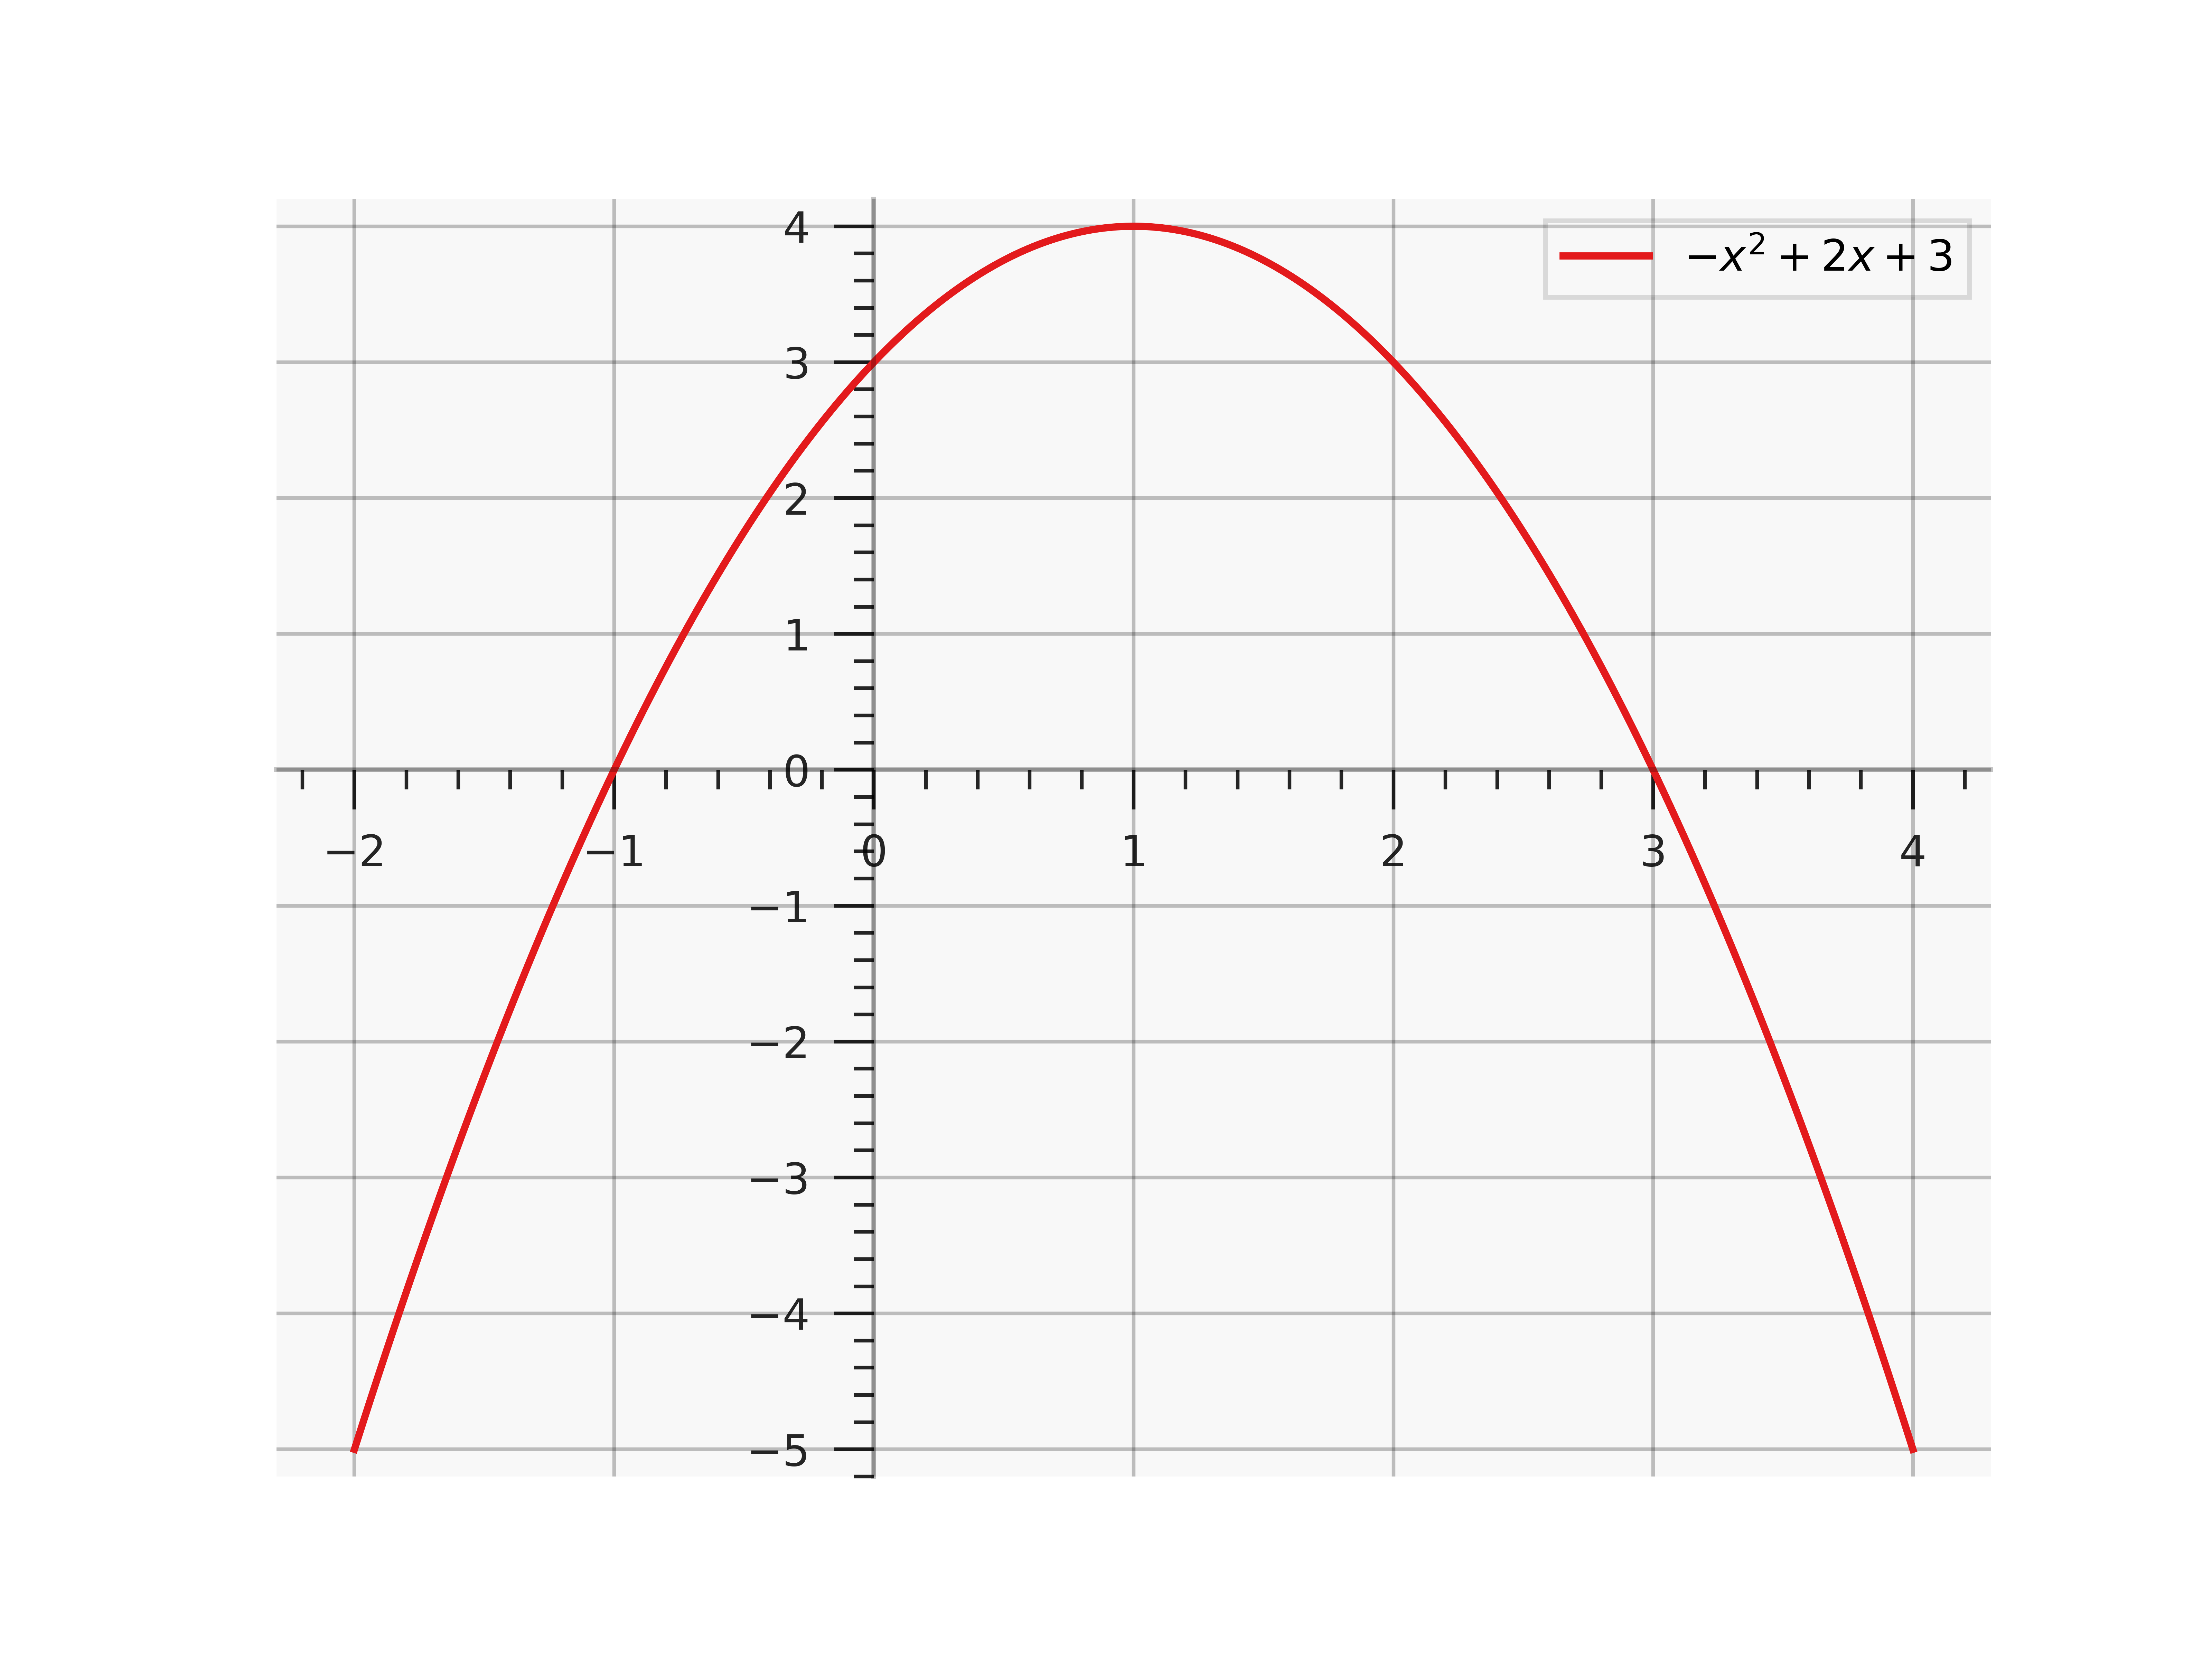
\includegraphics[width=10cm, keepaspectratio]{graph_3.png}
    \caption{Quadratic Functions}
    \label{fig:fig3}
\end{figure}

\begin{problem}
Graph $f(y) = y^2-6y+5$.
\end{problem}

This is a function of $y$ instead of $x$.
We can still graph this as a quadratic, but turned sideways.
Let's look at the function $f(x) = x^2-6x+5$ first.
We know that the parabola opens up and the vertex is $(3, -4)$.
With $y$ instead of $x$, everything will be inversed.

As $y$ goes away from the vertex point, the $x$ value will increase and thus the parabola will open up to the right.
The vertex will be $(-4, 3)$, as every point on the parabola given by $f(x)$ has its $x$ and $y$ coordinates swapped for $f(y)$.
Our sketch of the parabola is:

\begin{figure}[H]
    \centering
    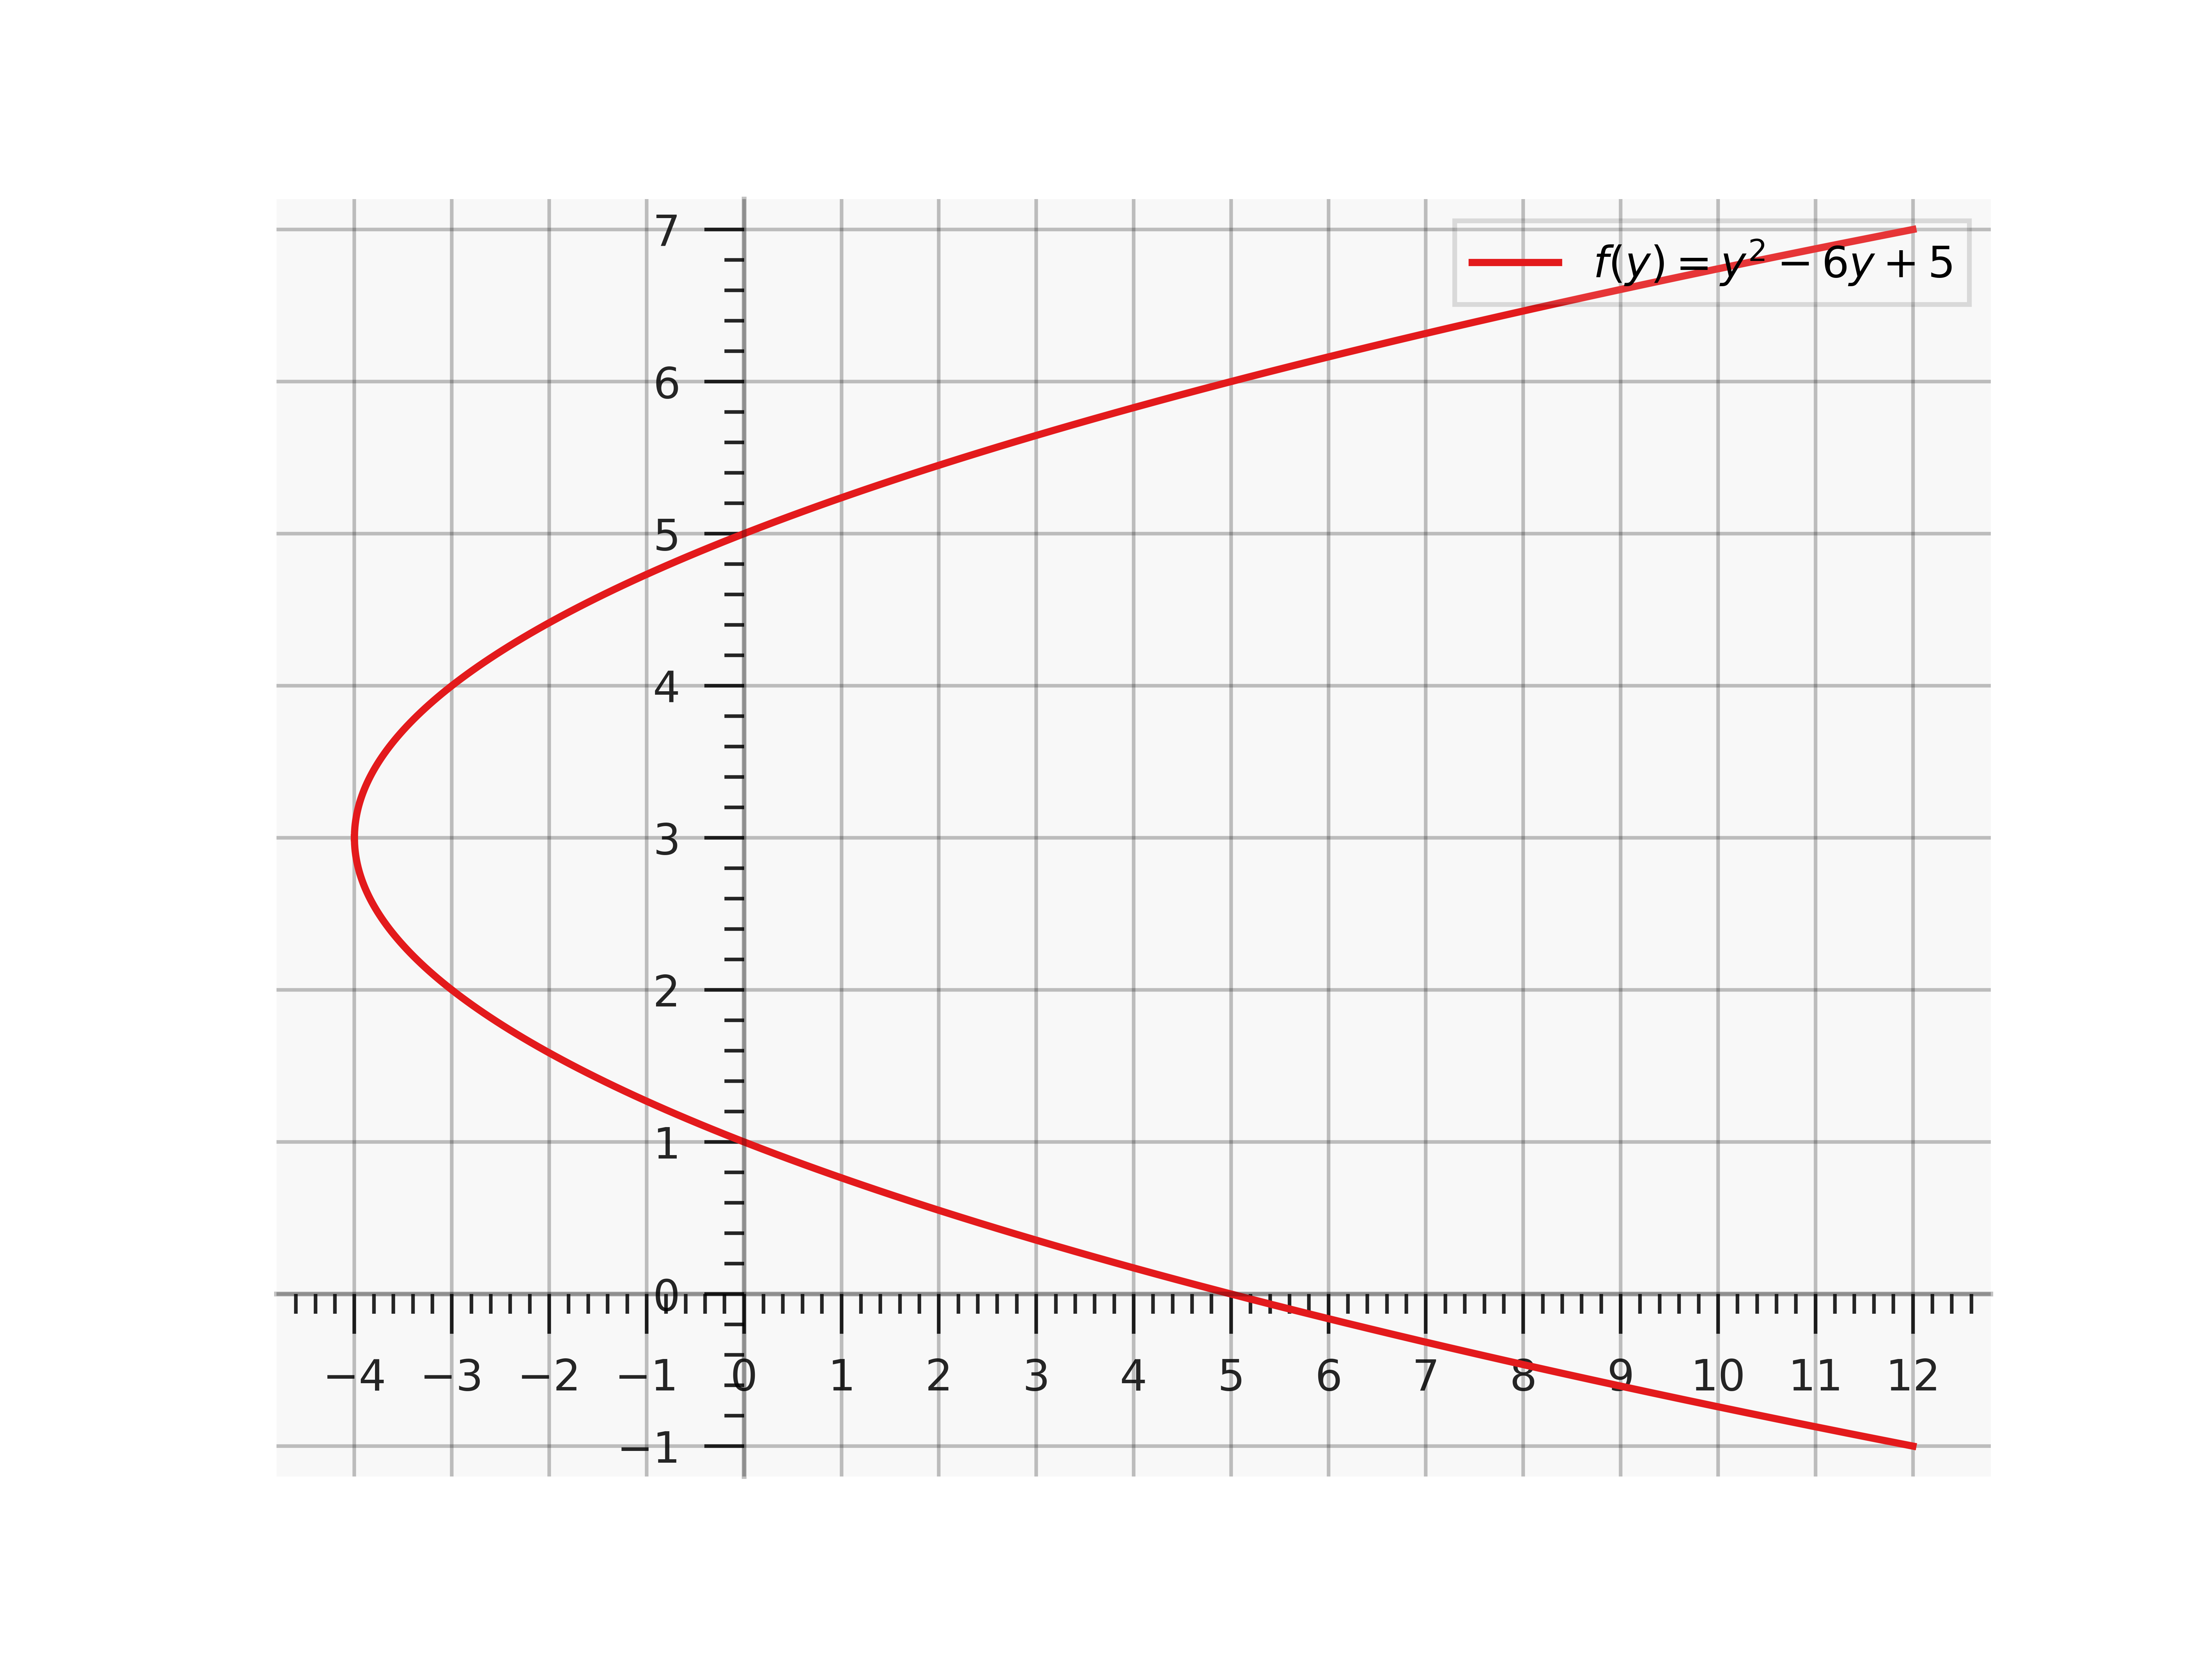
\includegraphics[width=10cm, keepaspectratio]{graph_4.png}
    \caption{Functions of $y$}
    \label{fig:fig4}
\end{figure}

\begin{problem}
Graph $x^2 + 2x + y^2 - 8y + 8 = 0$.
\end{problem}

We can put our equation above in a nicer form by completing the square for both the $x$ and $y$ terms.
This can be done as follows:

\begin{align}
    x^2 + 2x + y^2 - 8y + 8                   & = 0 \\
    x^2 + 2x + 1 - 1 + y^2 - 8y + 8 + 16 - 16 & = 0 \\
    (x+1)^2 + (y-4)^2 - 1 + 8 - 16            & = 0 \\
    (x+1)^2 + (y-4)^2                         & = 9
\end{align}

Now we can see that the equation represents a circle and is in standard form.

\begin{equation}
    (x-h)^2 + (y-k)^2 = r^2
\end{equation}

This allows us to easily identify the centre of the circle, $(h, k)$ and the radius of the circle, $r$.
Now we just need to sketch a circle with a radius of $3$ and a centre at $(-1, 4)$.

\begin{figure}[H]
    \centering
    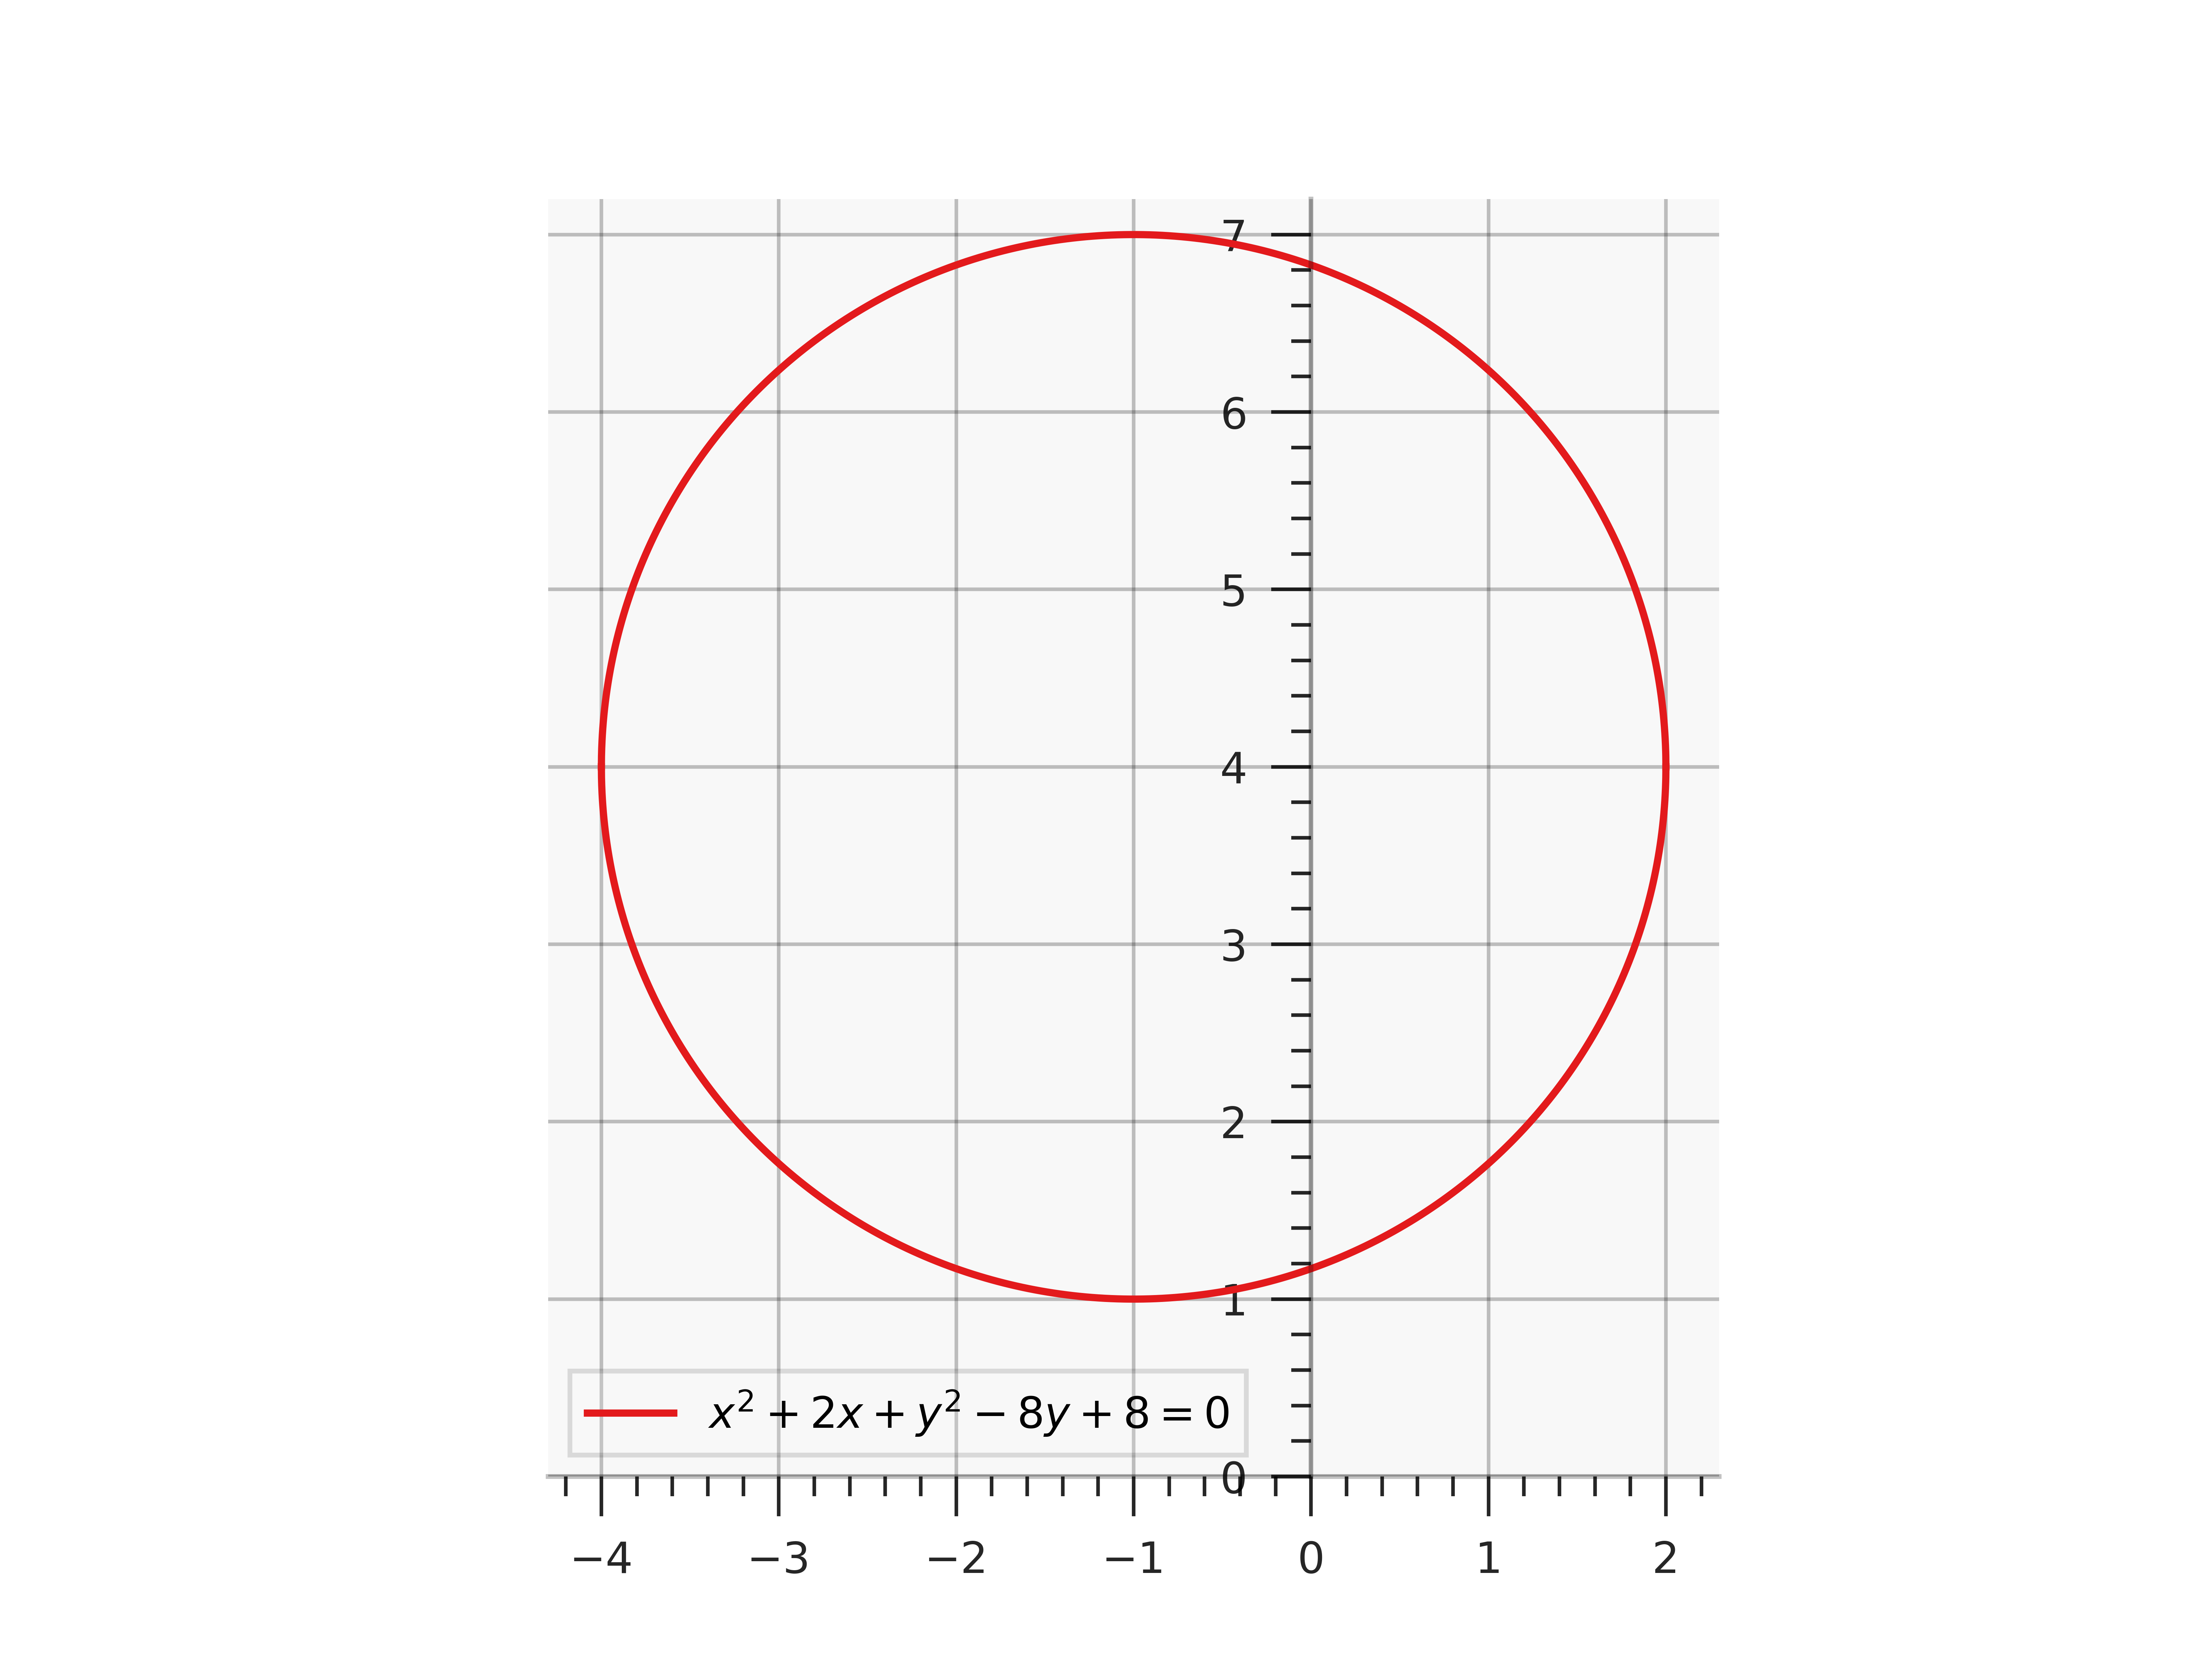
\includegraphics[width=10cm, keepaspectratio]{graph_5.png}
    \caption{Equation of a Circle}
    \label{fig:fig5}
\end{figure}

\begin{problem}
Graph $\displaystyle \frac{(x-2)^2}{9} + 4(y + 2 )^2 = 1$.
\end{problem}

This describes an ellipse. The standard form for the equation of an ellipse is:

\begin{equation}
    \frac{(x - h)^2}{a} + \frac{(y - k)^2}{b} = 1
\end{equation}

For our equation, $b^2$ would simply be $\frac{1}{4}$.
The centre of the ellipse is $(h, k)$.
$a$ is the distance between the centre and the topmost or bottommost points on the ellipse while $b$ is the distance between the centre and the rightmost or leftmost points on the ellipse.

Our ellipse has a centre of $(2, -2)$ and $a=3$ and $b=\frac{1}{2}$.
The graph is then:

\begin{figure}[H]
    \centering
    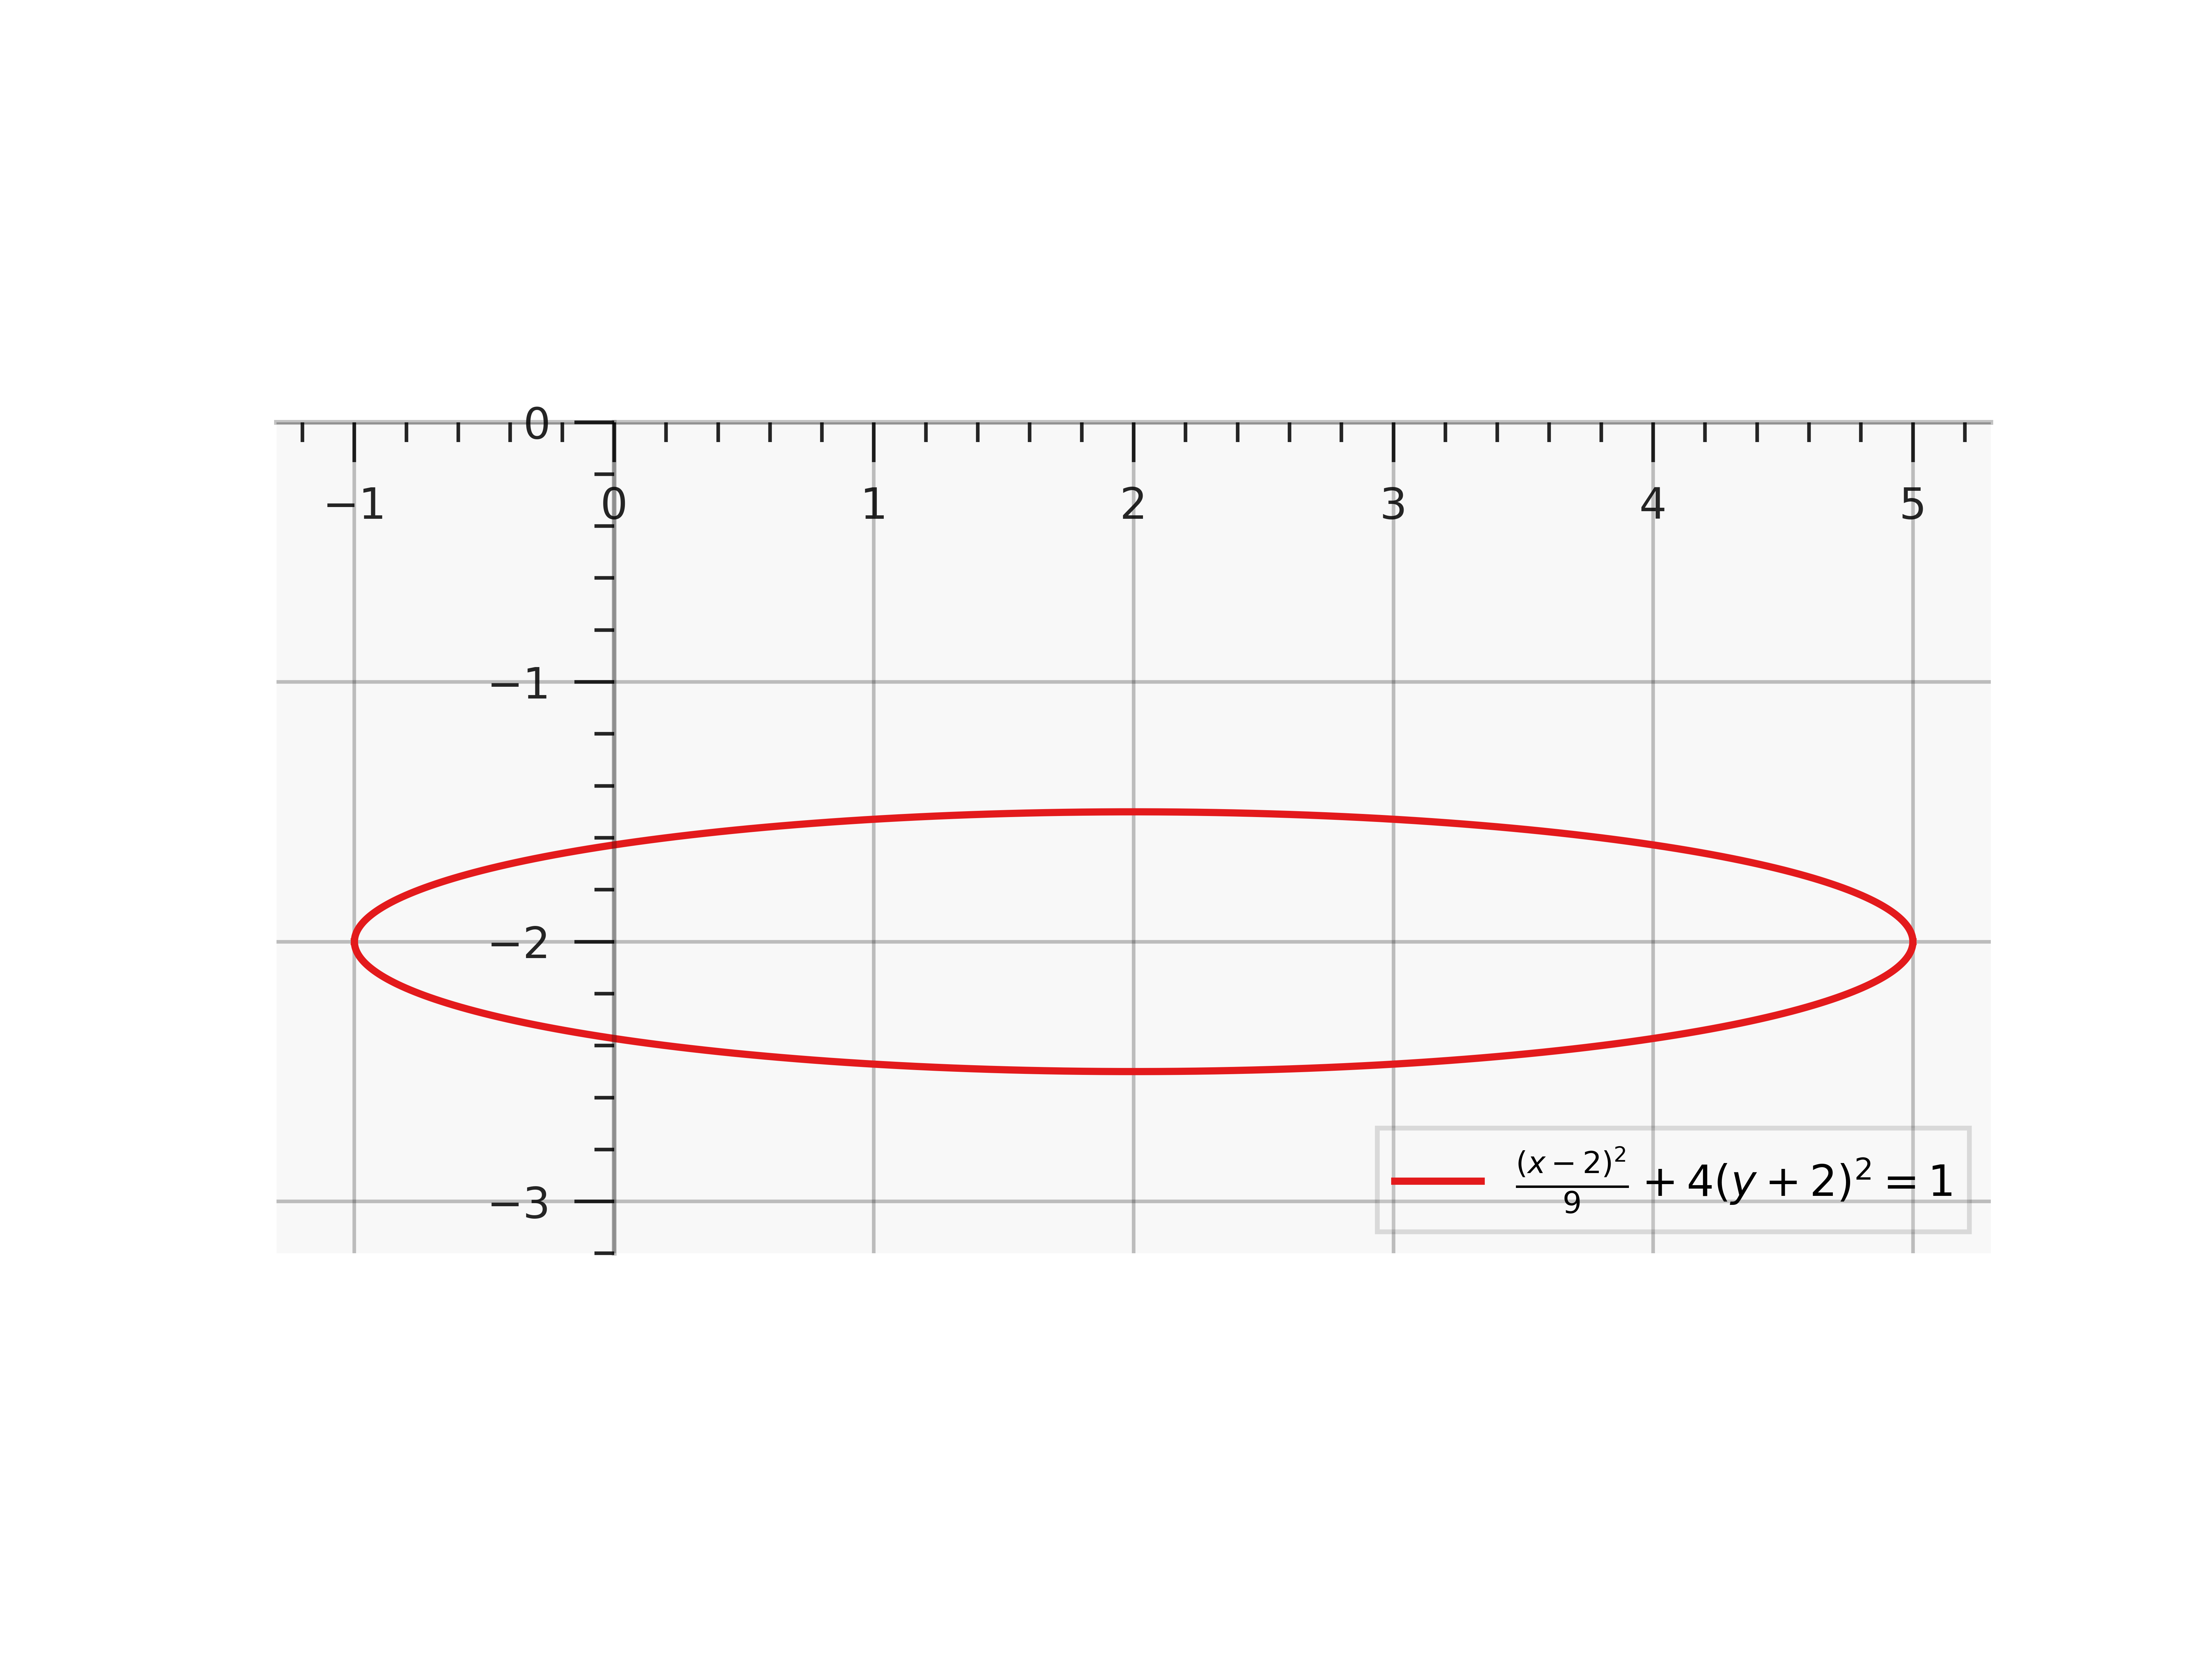
\includegraphics[width=10cm, keepaspectratio]{graph_6.png}
    \caption{Equation of an Ellipse}
    \label{fig:fig6}
\end{figure}

\begin{problem}
Graph $\displaystyle \frac{(x+1)^2}{9} - \frac{(y-2)^2}{4} = 1$.
\end{problem}

This is an equation for a hyperbola.
There are two standard forms of the equations for a hyperbola.

\begin{equation}
    \frac{(x-h)^2}{a^2} - \frac{(y-k)^2}{b^2} = 1 \qquad \qquad \frac{(x-h)^2}{b^2} - \frac{(y-k)^2}{a^2} = 1
\end{equation}

Hyperbolas of the first form have a centre at $(h,k)$ and open to the right and left.
They have vertices $a$ units to the right and left from their centre and the gradient of their asymptotes is $\pm\frac{b}{a}$.
Hyperbolas of the second form also have a centre at $(h,k)$ but open upwards and downwards from their centre.
They have vertices $b$ units up and down from the centre and the gradient of their asymptotes is also $\pm\frac{b}{a}$.

Our hyperbola has a centre at $(-1, 2)$.
The centre of the hyperbola acts more as a starting point from where it is drawn.
The hyperbola will open to the left and right as the $x$ term is positive.
The asymptotes wll have slopes $\pm\frac{2}{3}$.
The asymptotes are two lines which intersect at the origin and are what the two branches of the hyperbola will approach as $x$ goes to $\infty$ and $-\infty$.

The sketch of the hyperbola (and the asymptote lines) is then:

\begin{figure}[H]
    \centering
    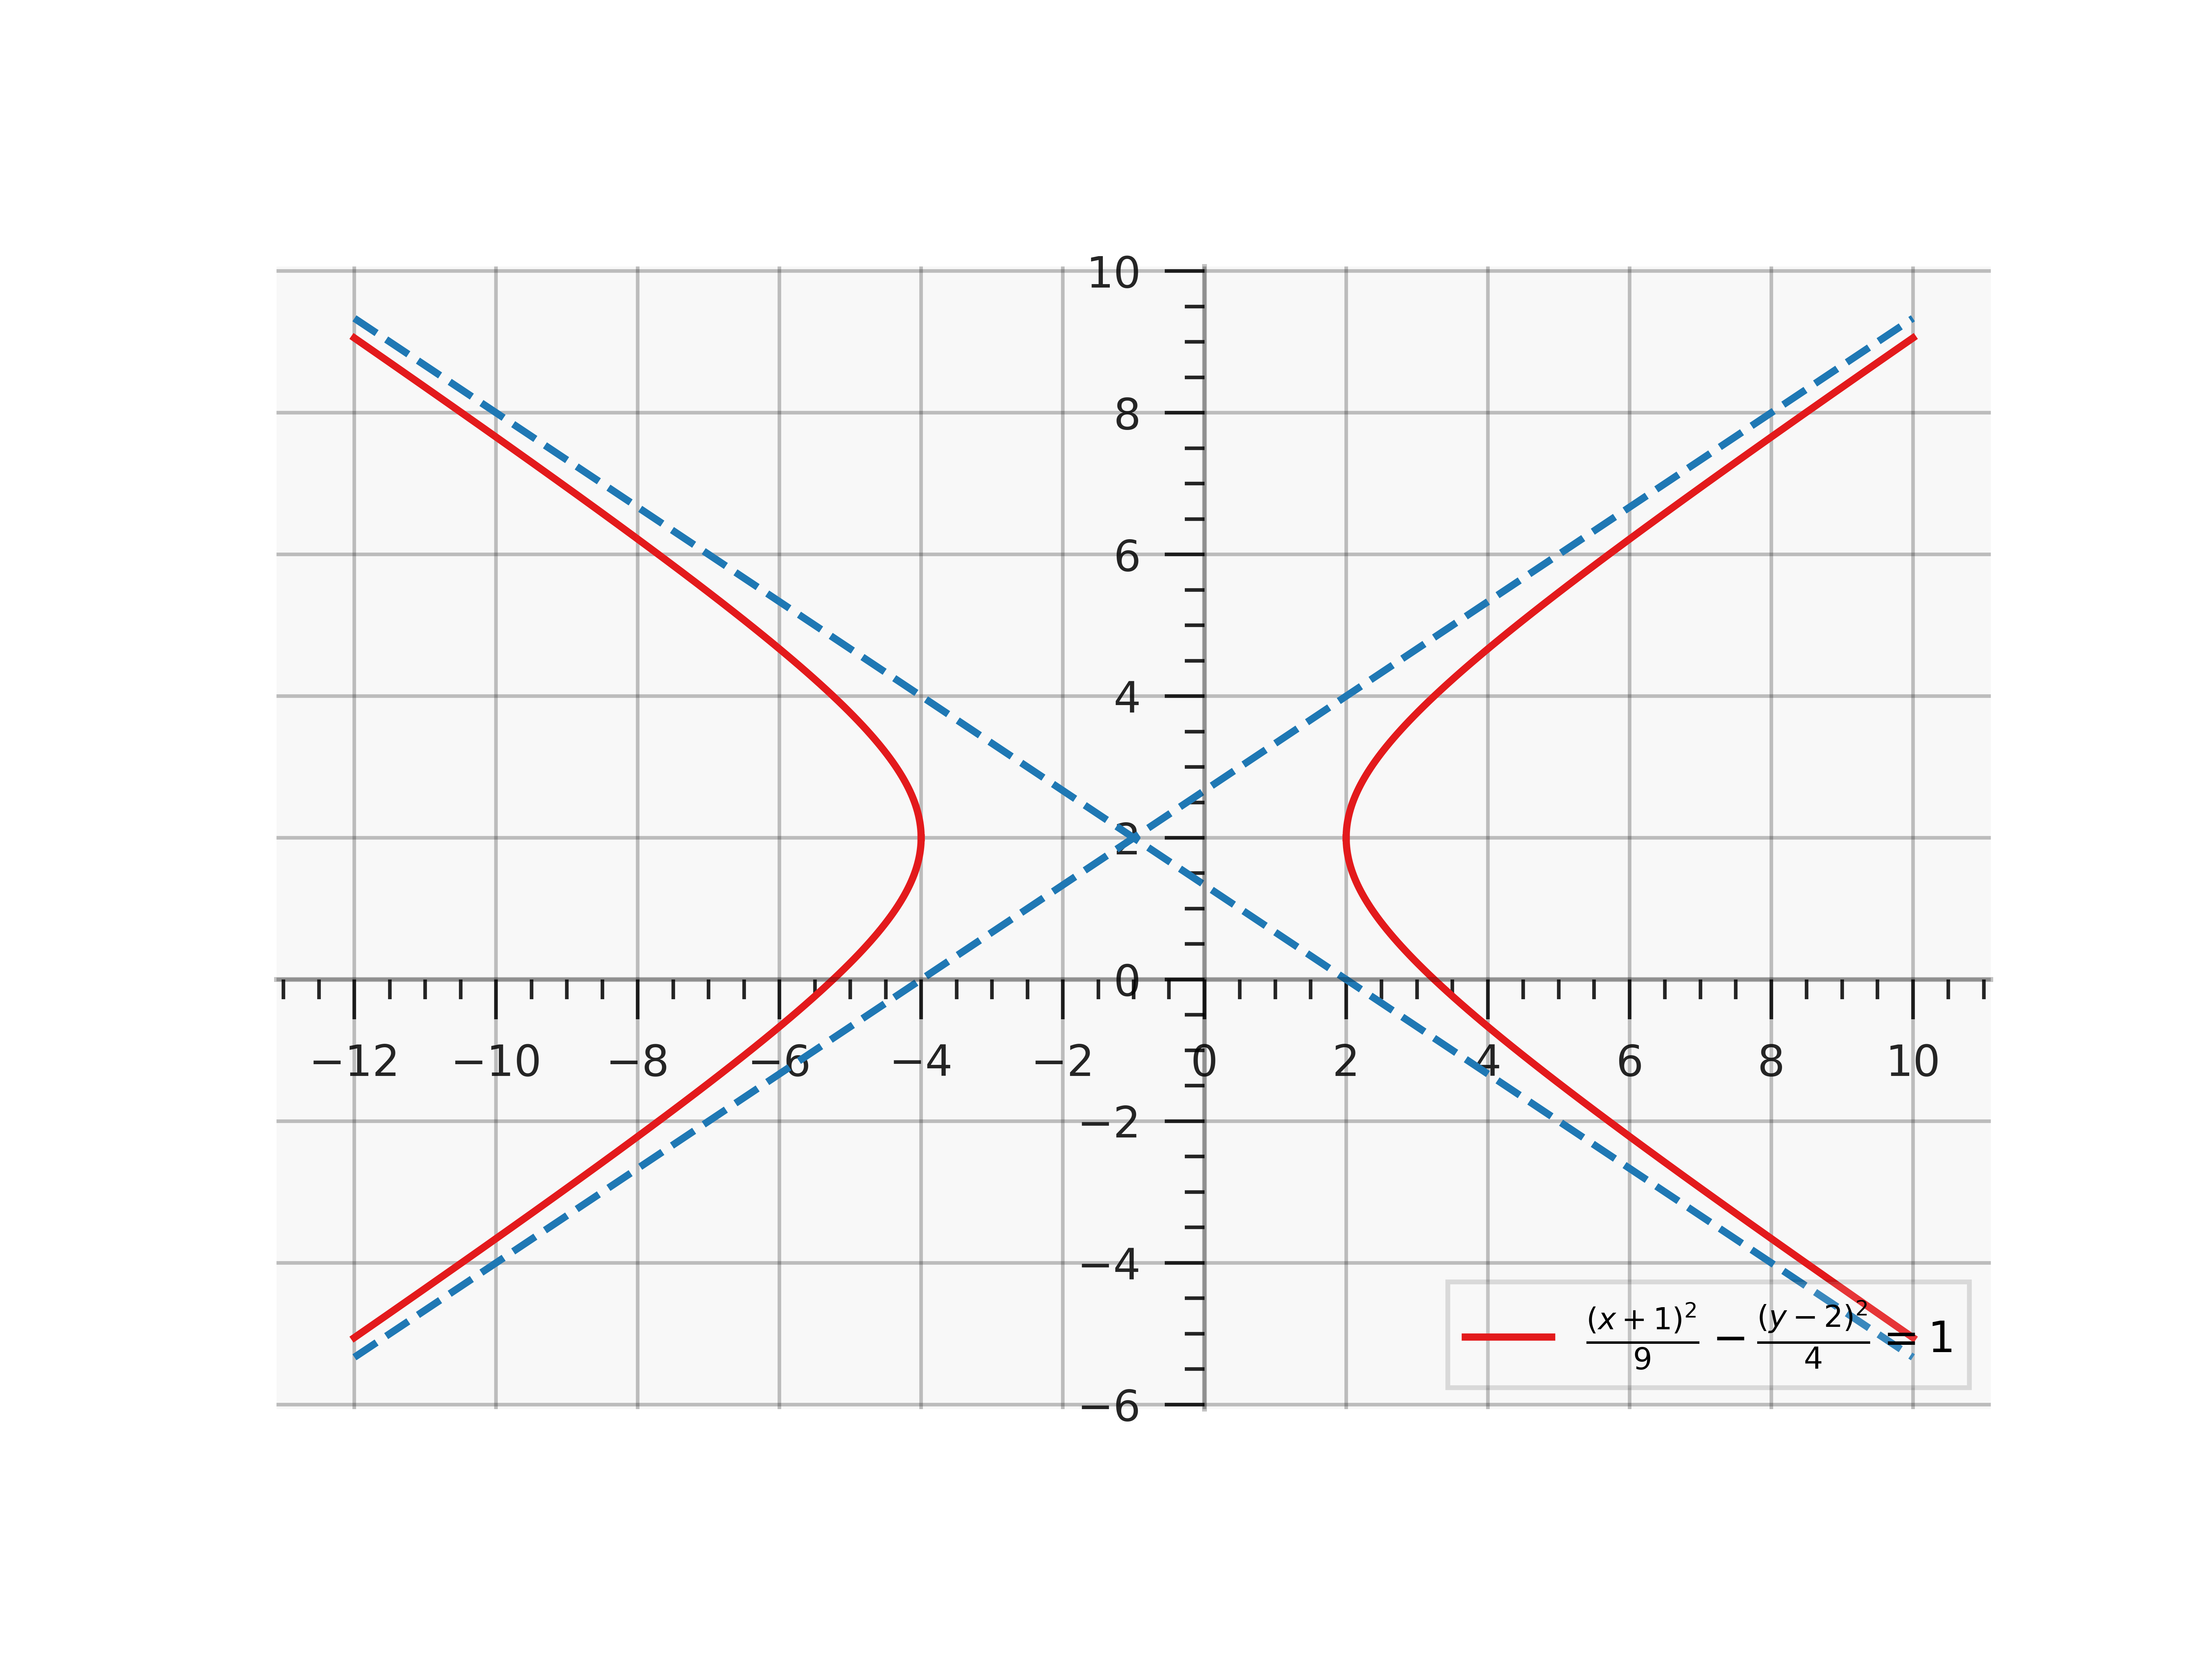
\includegraphics[width=10cm, keepaspectratio]{graph_7.png}
    \caption{Equation of a Hyperbola}
    \label{fig:fig7}
\end{figure}

\begin{problem}
Graph $f(x)=e^x$ and $g(x)=e^{-x}$.
\end{problem}

Exponential functions show up regularly in Calculus and their behaviour as $x$ goes to $\infty$ and $-\infty$ is important.
We can clearly see their behaviour from their graphs, which may sketched as shown below:

\begin{figure}[H]
    \centering
    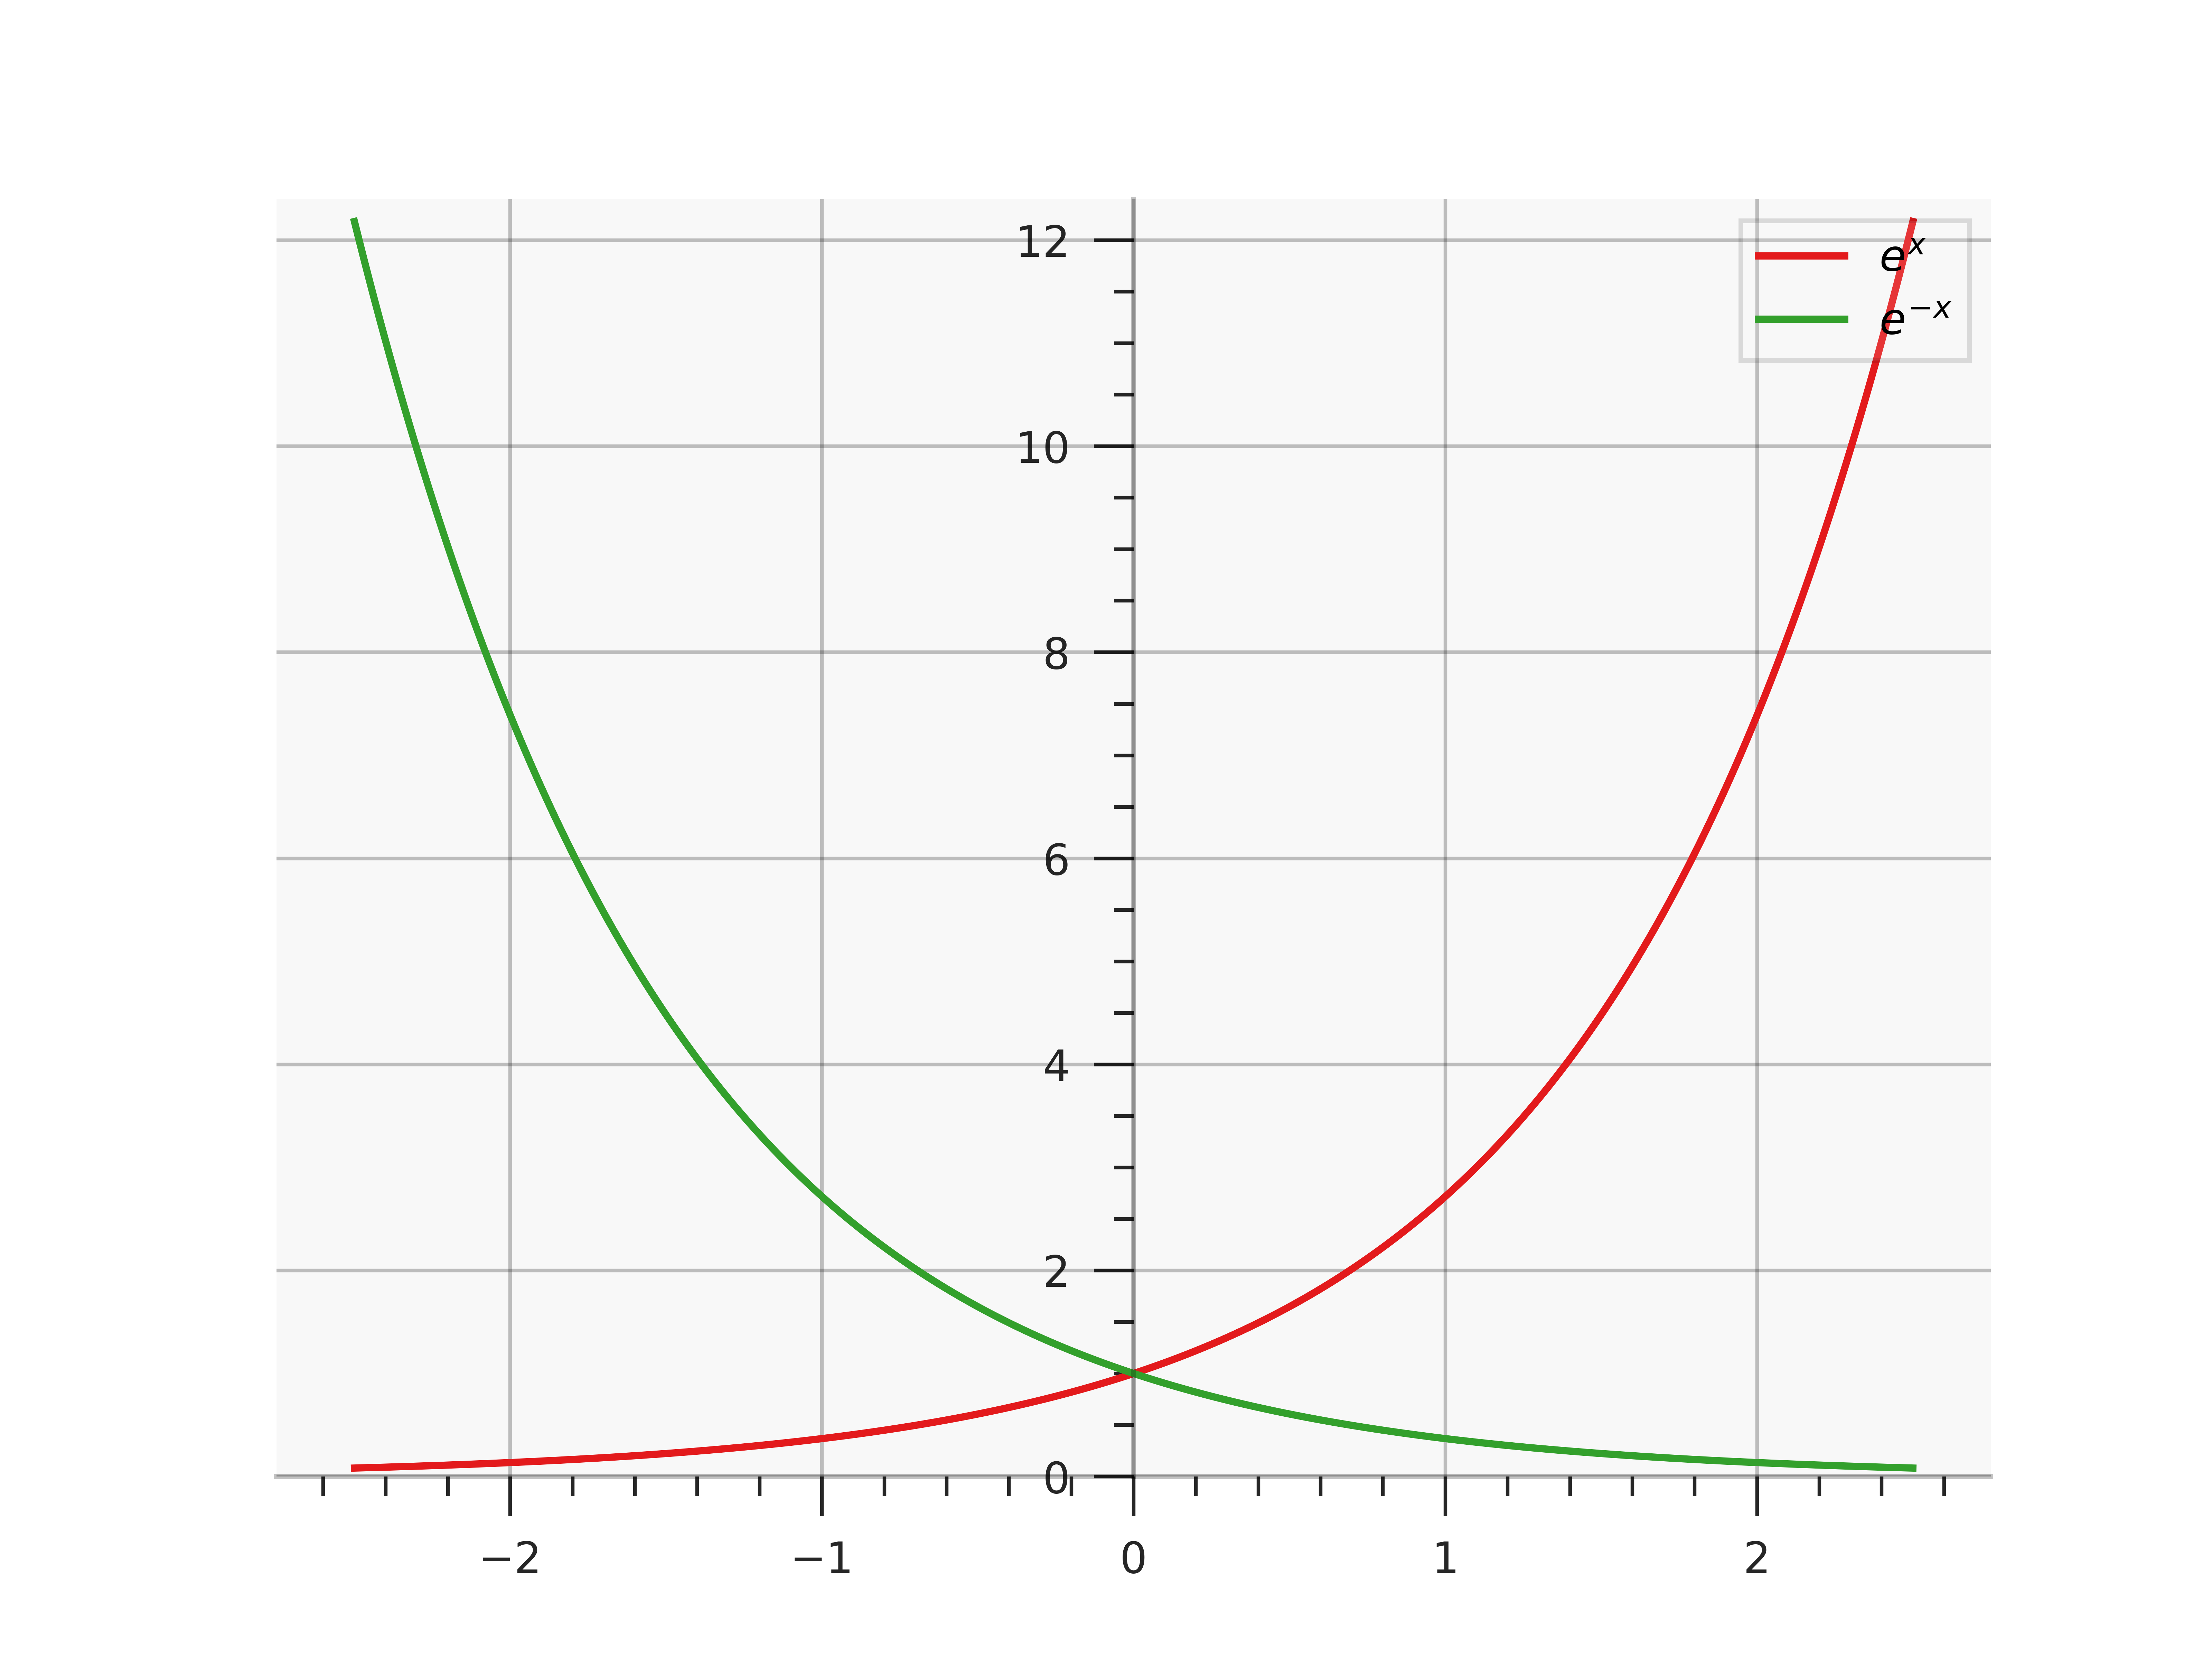
\includegraphics[width=10cm, keepaspectratio]{graph_8.png}
    \caption{Exponential Functions}
    \label{fig:fig8}
\end{figure}

\begin{problem}
Graph $f(x)=\ln(x)$.
\end{problem}

This is rather simple and has been graphed in an earlier review section.
However, it is important enough to be here.
The sketch of the natural logarithm function is below:

\begin{figure}[H]
    \centering
    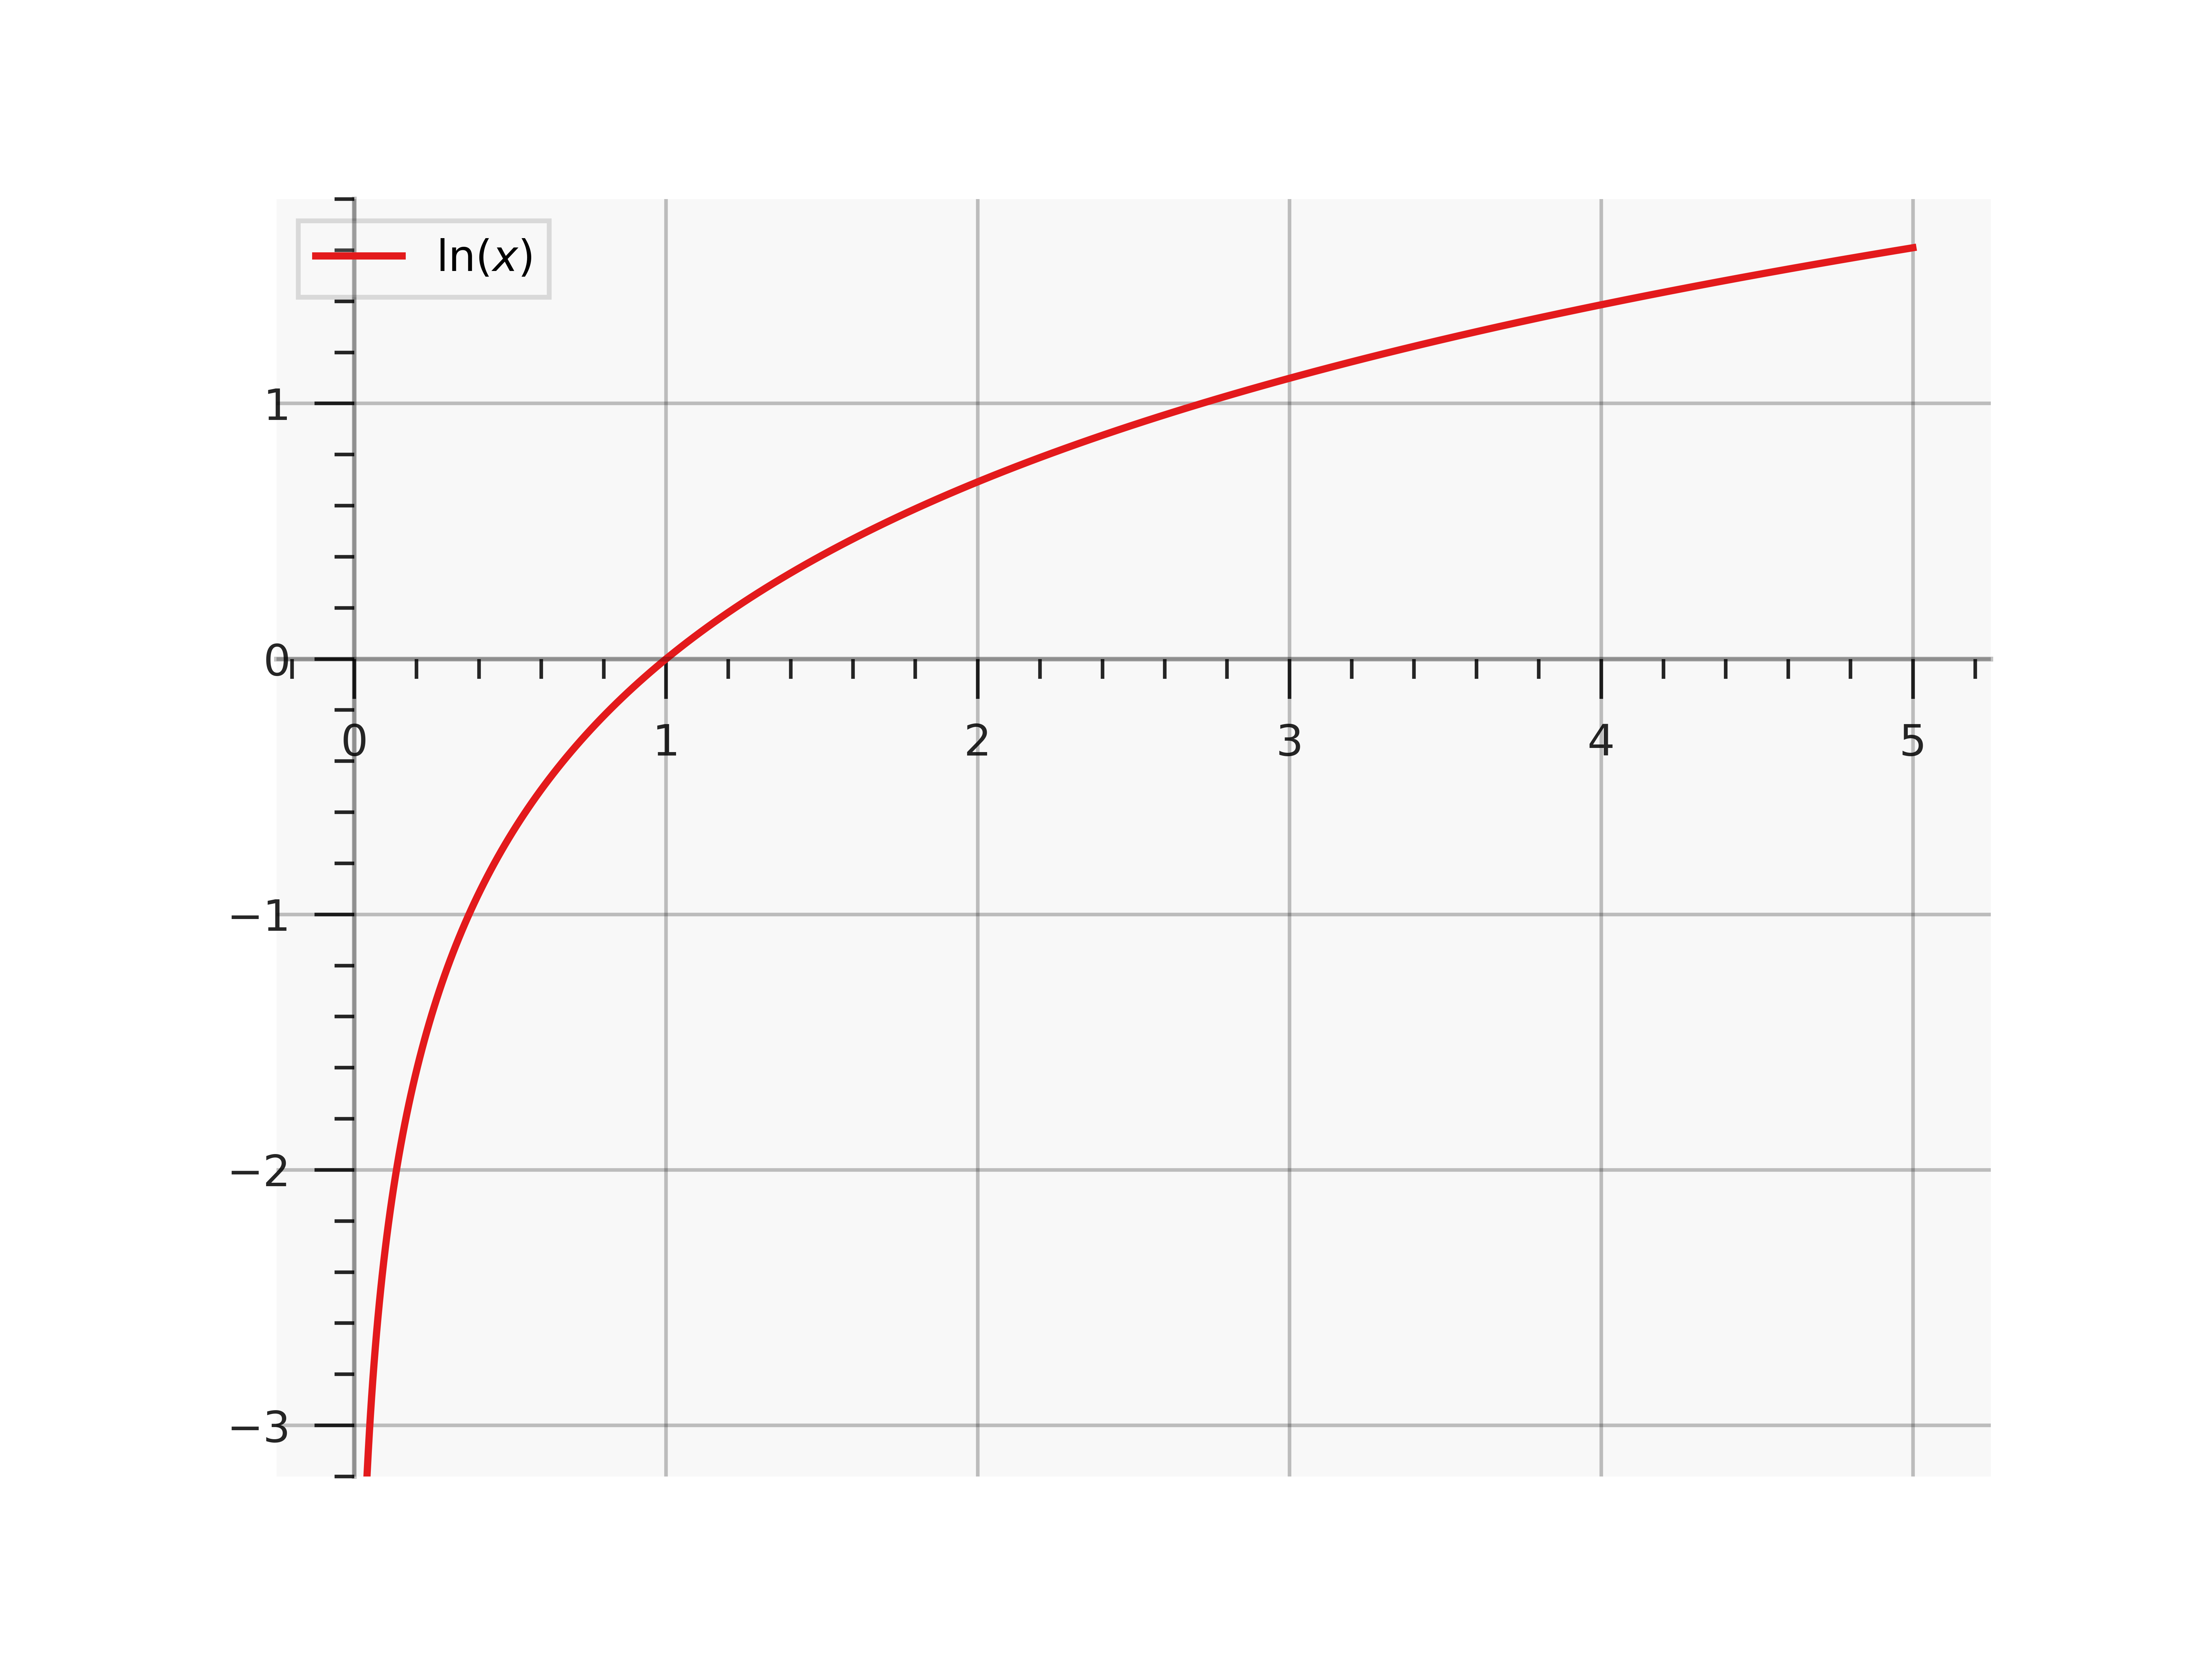
\includegraphics[width=10cm, keepaspectratio]{graph_9.png}
    \caption{Logarithmic Functions}
    \label{fig:fig9}
\end{figure}

\begin{problem}
Graph $f(x)=\sqrt{x}$.
\end{problem}

This is another simple function that is quite common.
One thing to remember is that the domain of the square root function is $x\geq 0$.
Our sketch is:

\begin{figure}[H]
    \centering
    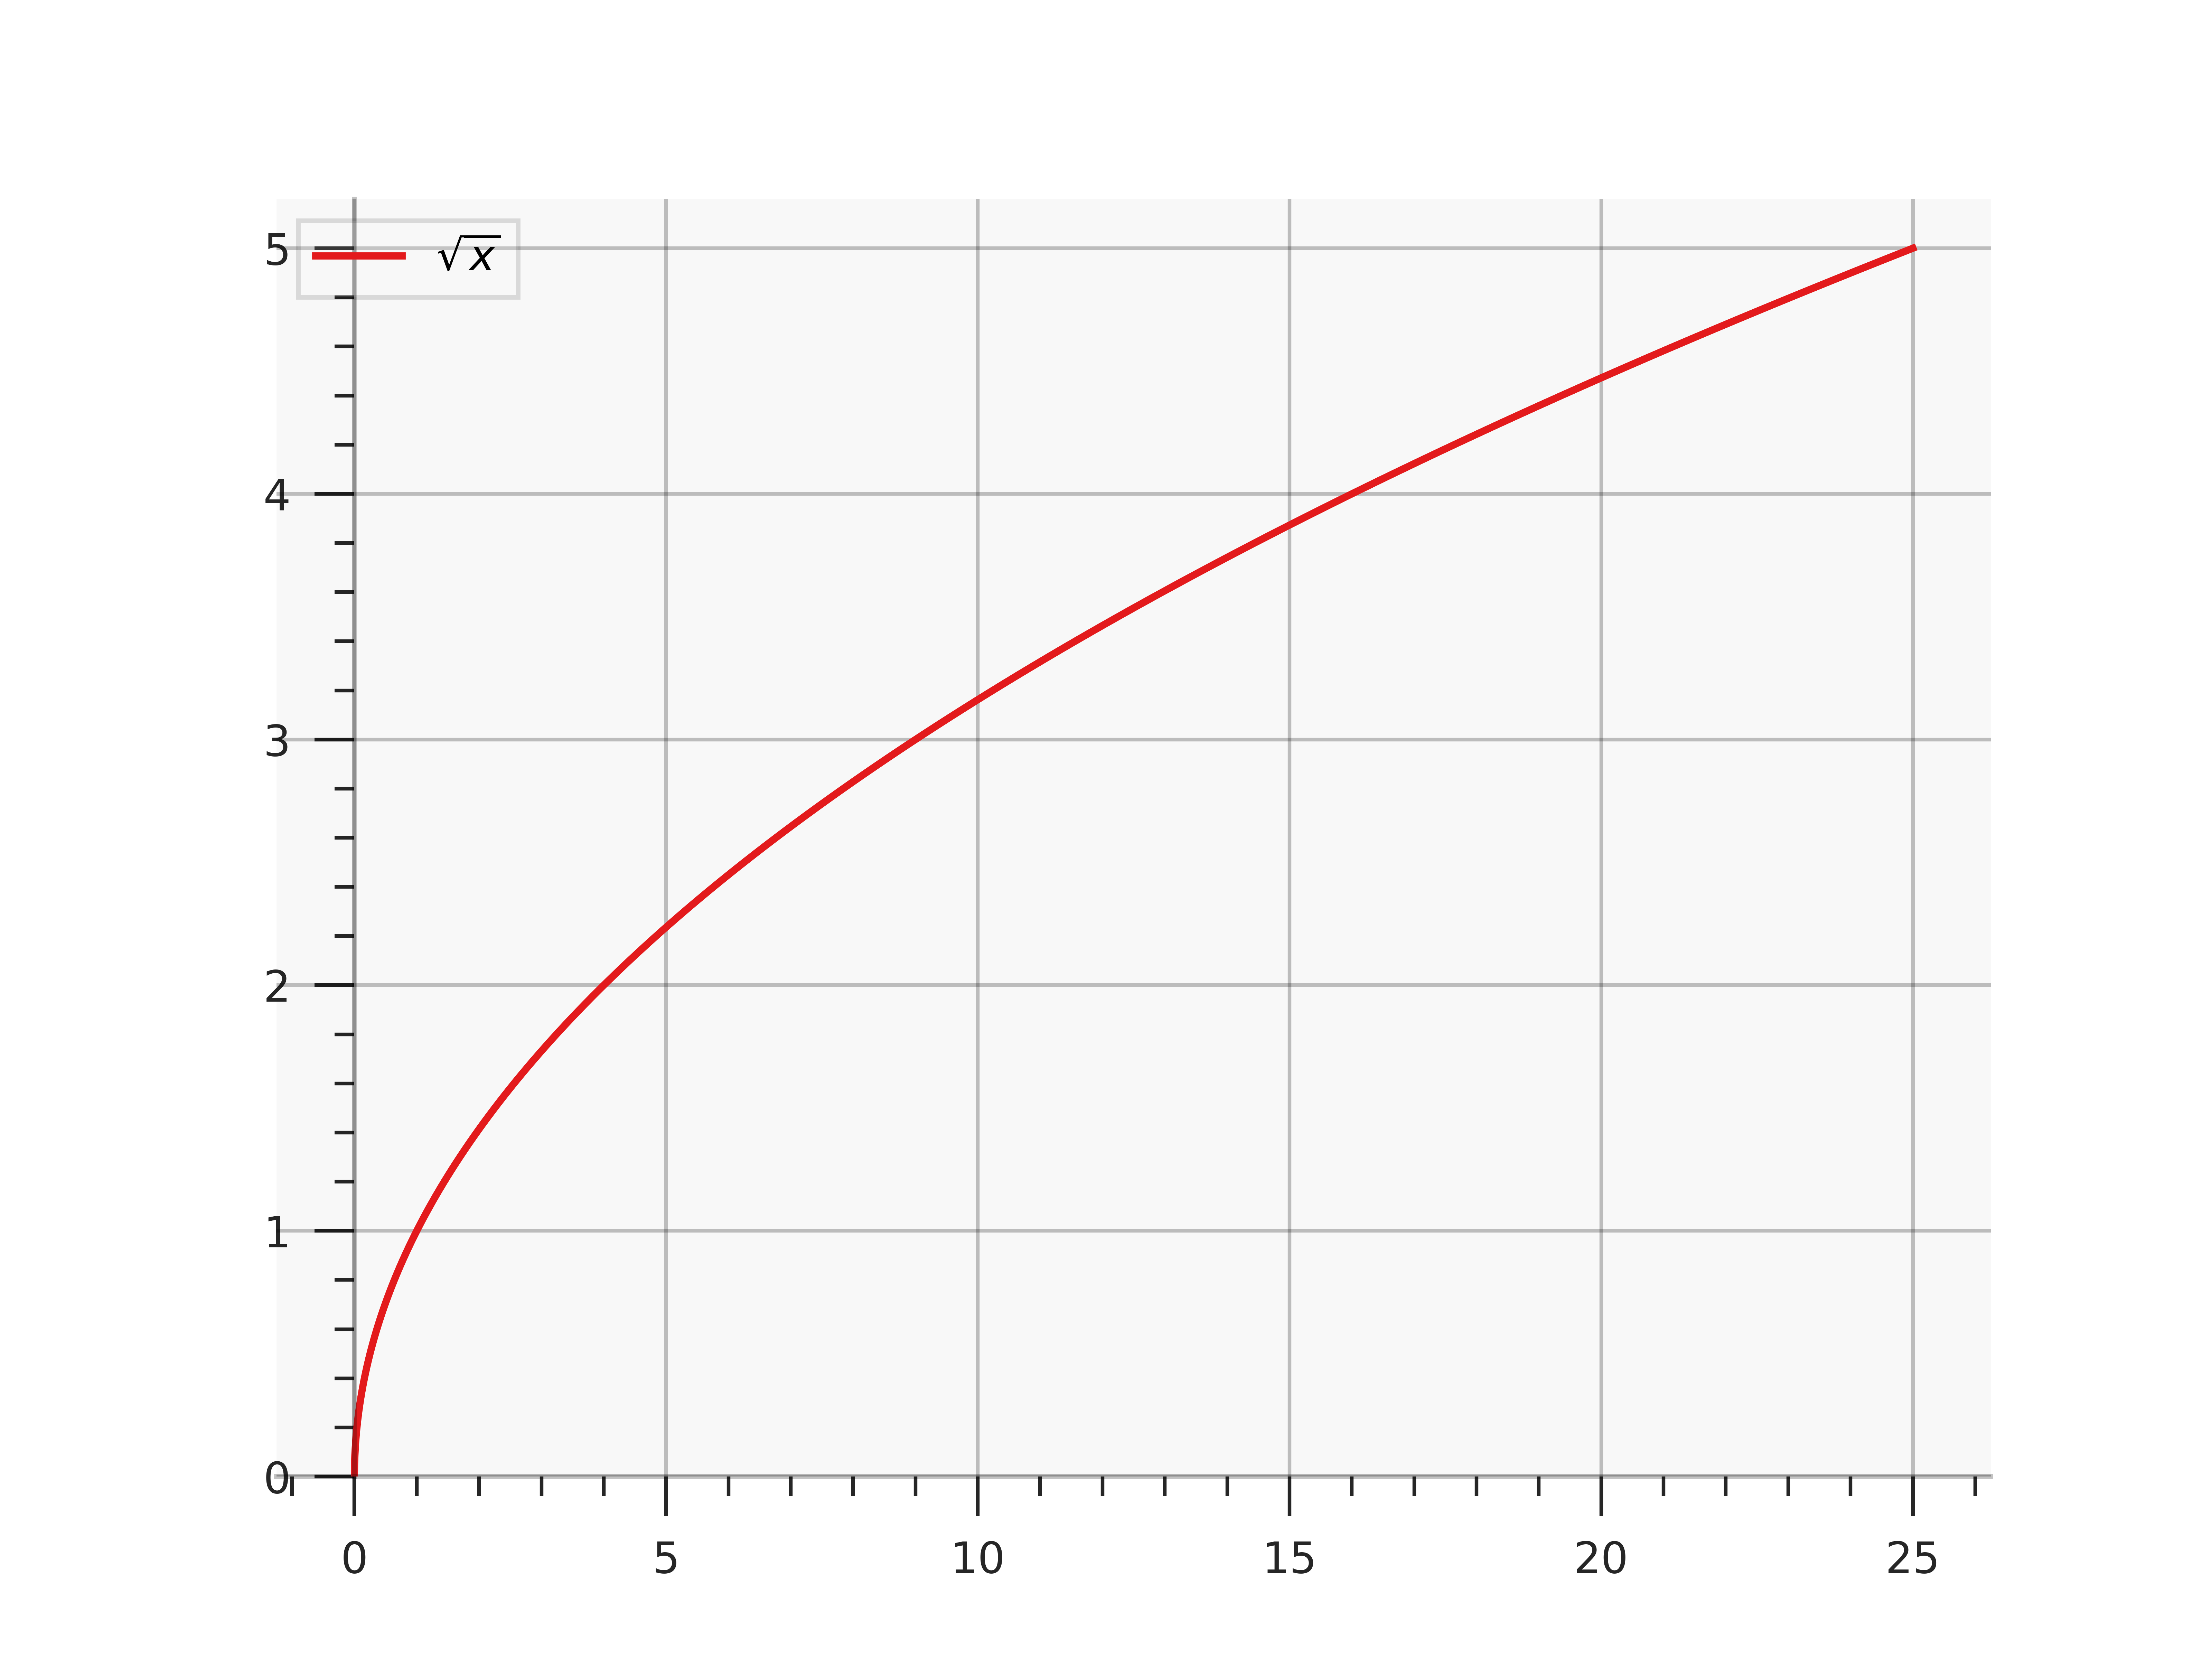
\includegraphics[width=10cm, keepaspectratio]{graph_10.png}
    \caption{Radical Functions}
    \label{fig:fig10}
\end{figure}

\begin{problem}
Graph $f(x)=x^3$.
\end{problem}

This is another simple function and there isn't too much too do.
It is a common polynomial however.
The sketch is:

\begin{figure}[H]
    \centering
    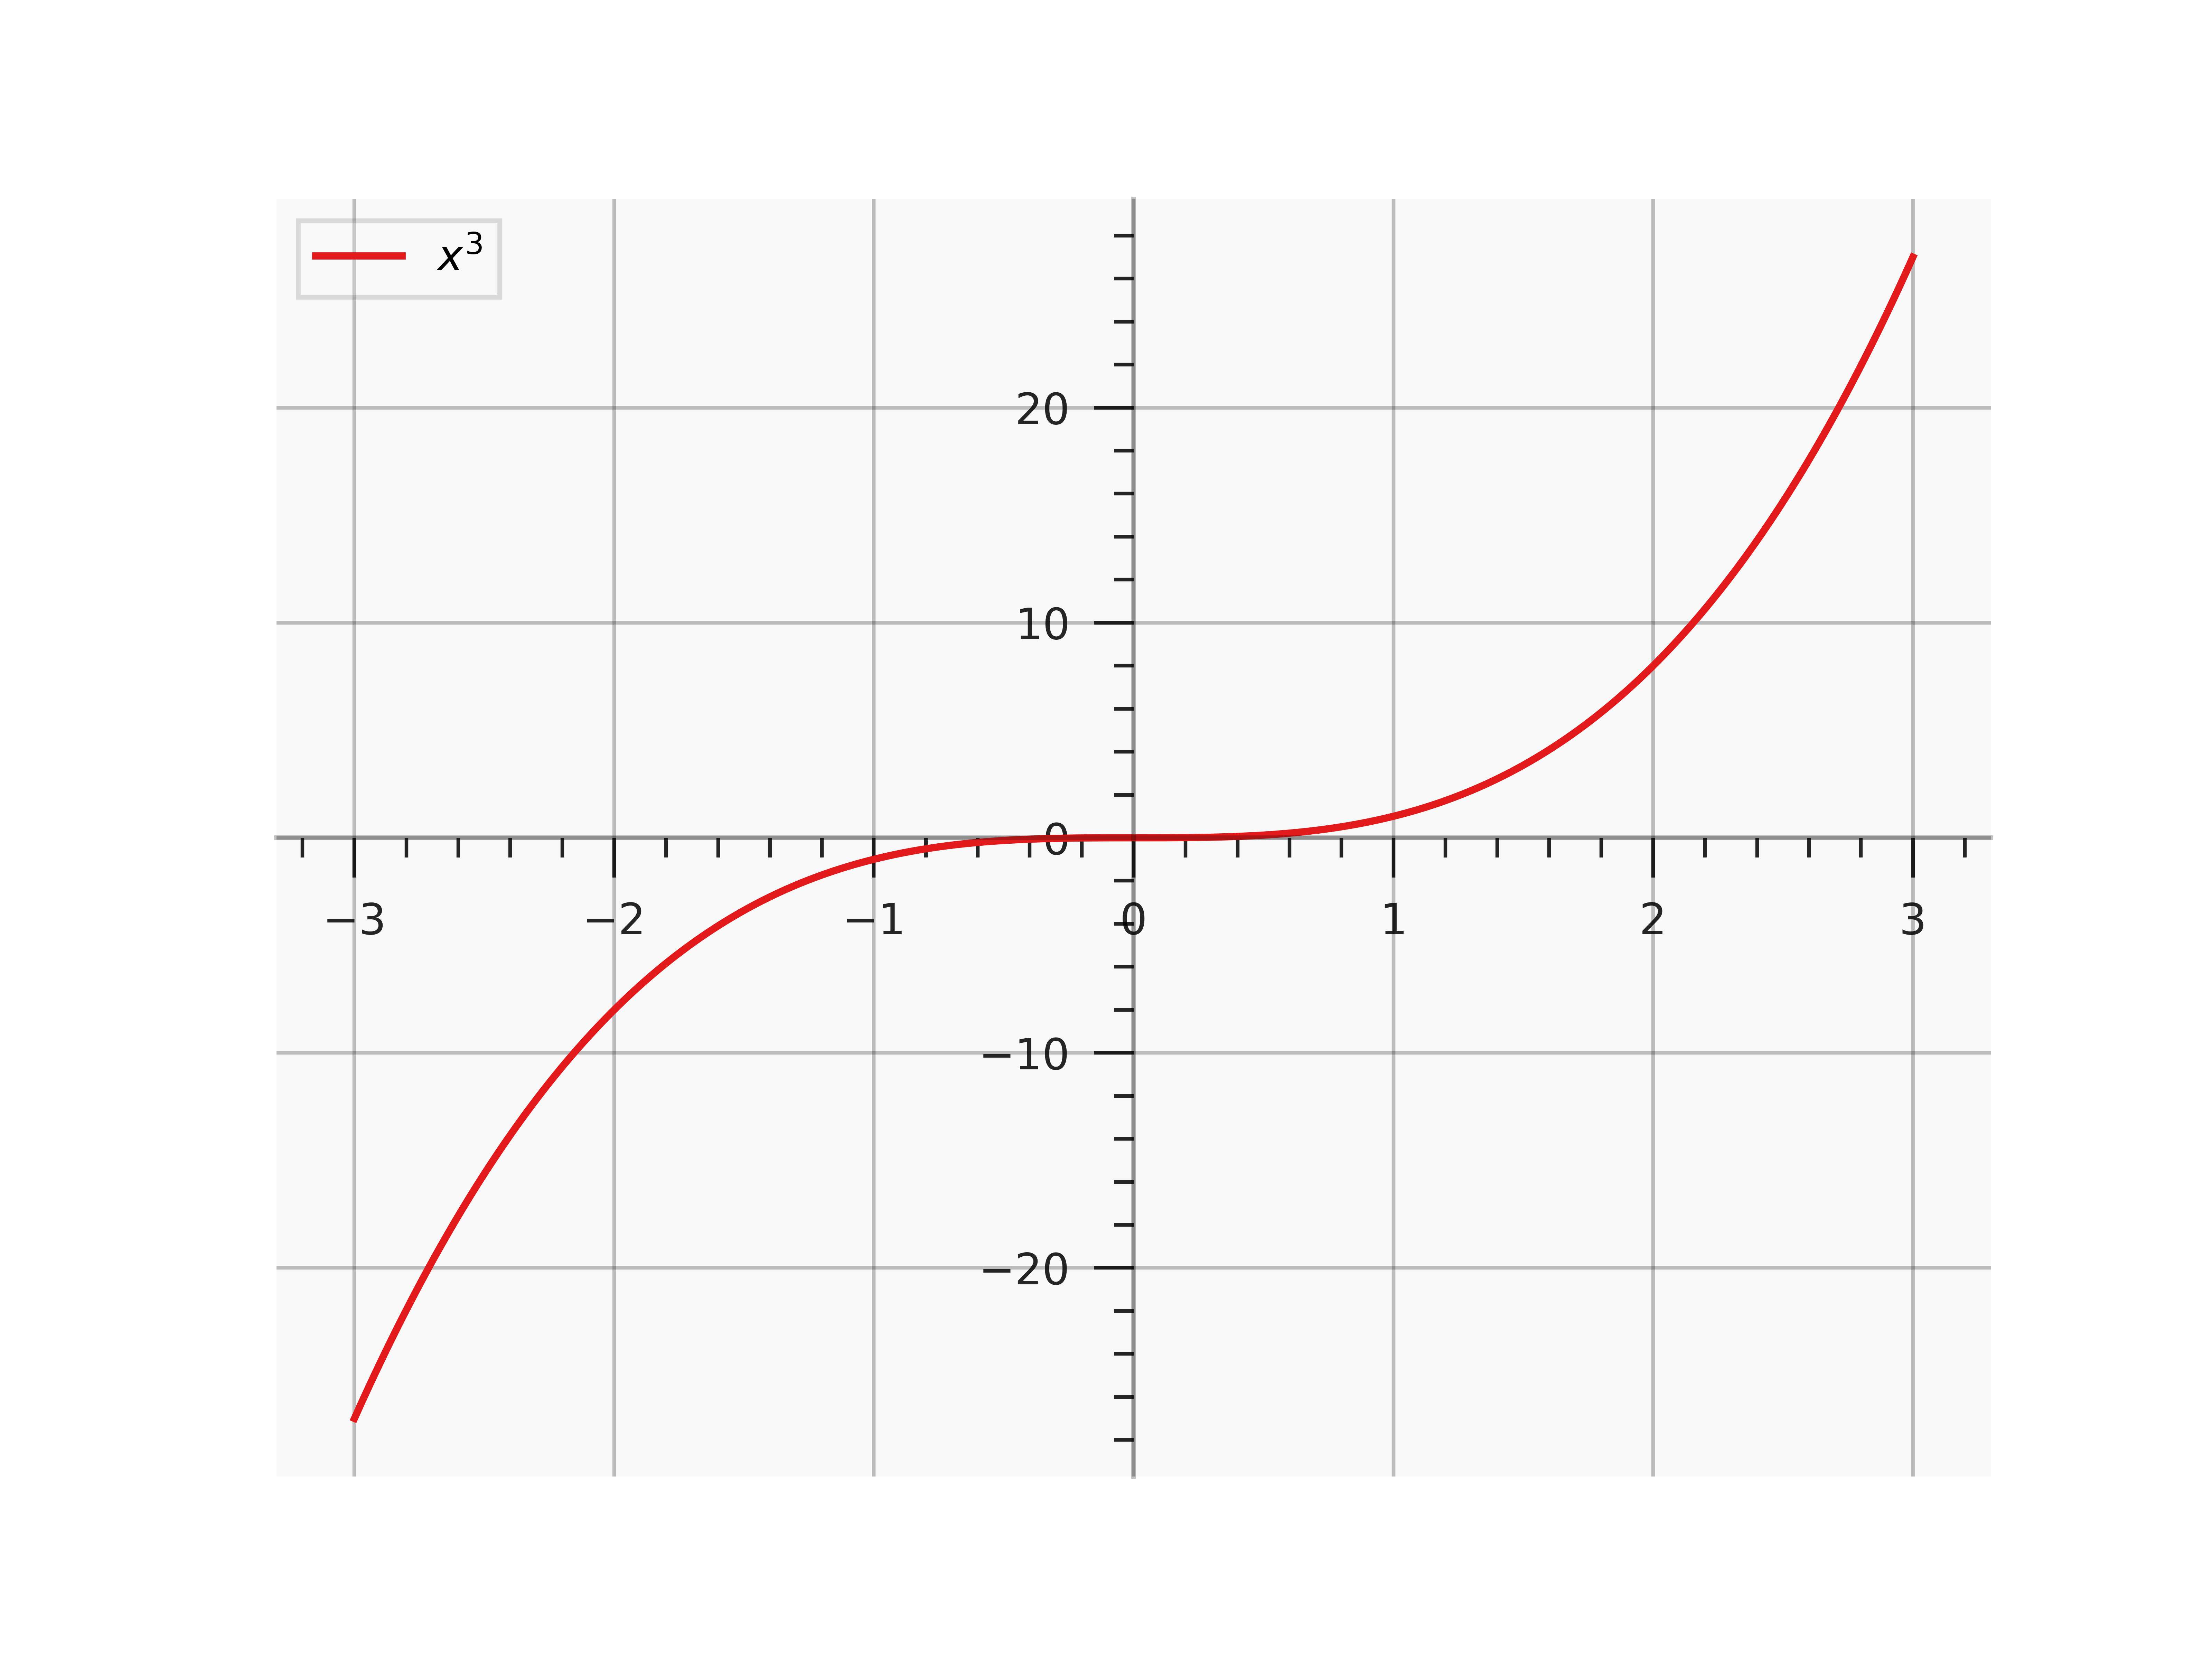
\includegraphics[width=10cm, keepaspectratio]{graph_11.png}
    \caption{Cubic Functions}
    \label{fig:fig11}
\end{figure}

\begin{problem}
Graph $f(x)=\cos(x)$.
\end{problem}

This is a rather simple trigonometric function.
Note that we are able to plug in any value into the cosine function, which is note true for all trig functions.
Then, we can say that the domain of $\cos(x)$ is $\mathbb{R}$, the set of real numbers.
Another thing to note is:

\begin{equation}
    -1 \leq \cos(x) \leq 1
\end{equation}

The cosine of some number will never be greater than 1 or less than $-1$.
This may be useful occasionally in Calculus.
In general, we may say that:

\begin{equation}
    -A \leq A\cos(\omega x) \leq A
\end{equation}

Below is the sketch of $\cos(x)$ for the interval $-4\pi \leq x \leq 4\pi$.
The $x$ values are in radians and not degrees as is commonplace in Calculus.

\begin{figure}[H]
    \centering
    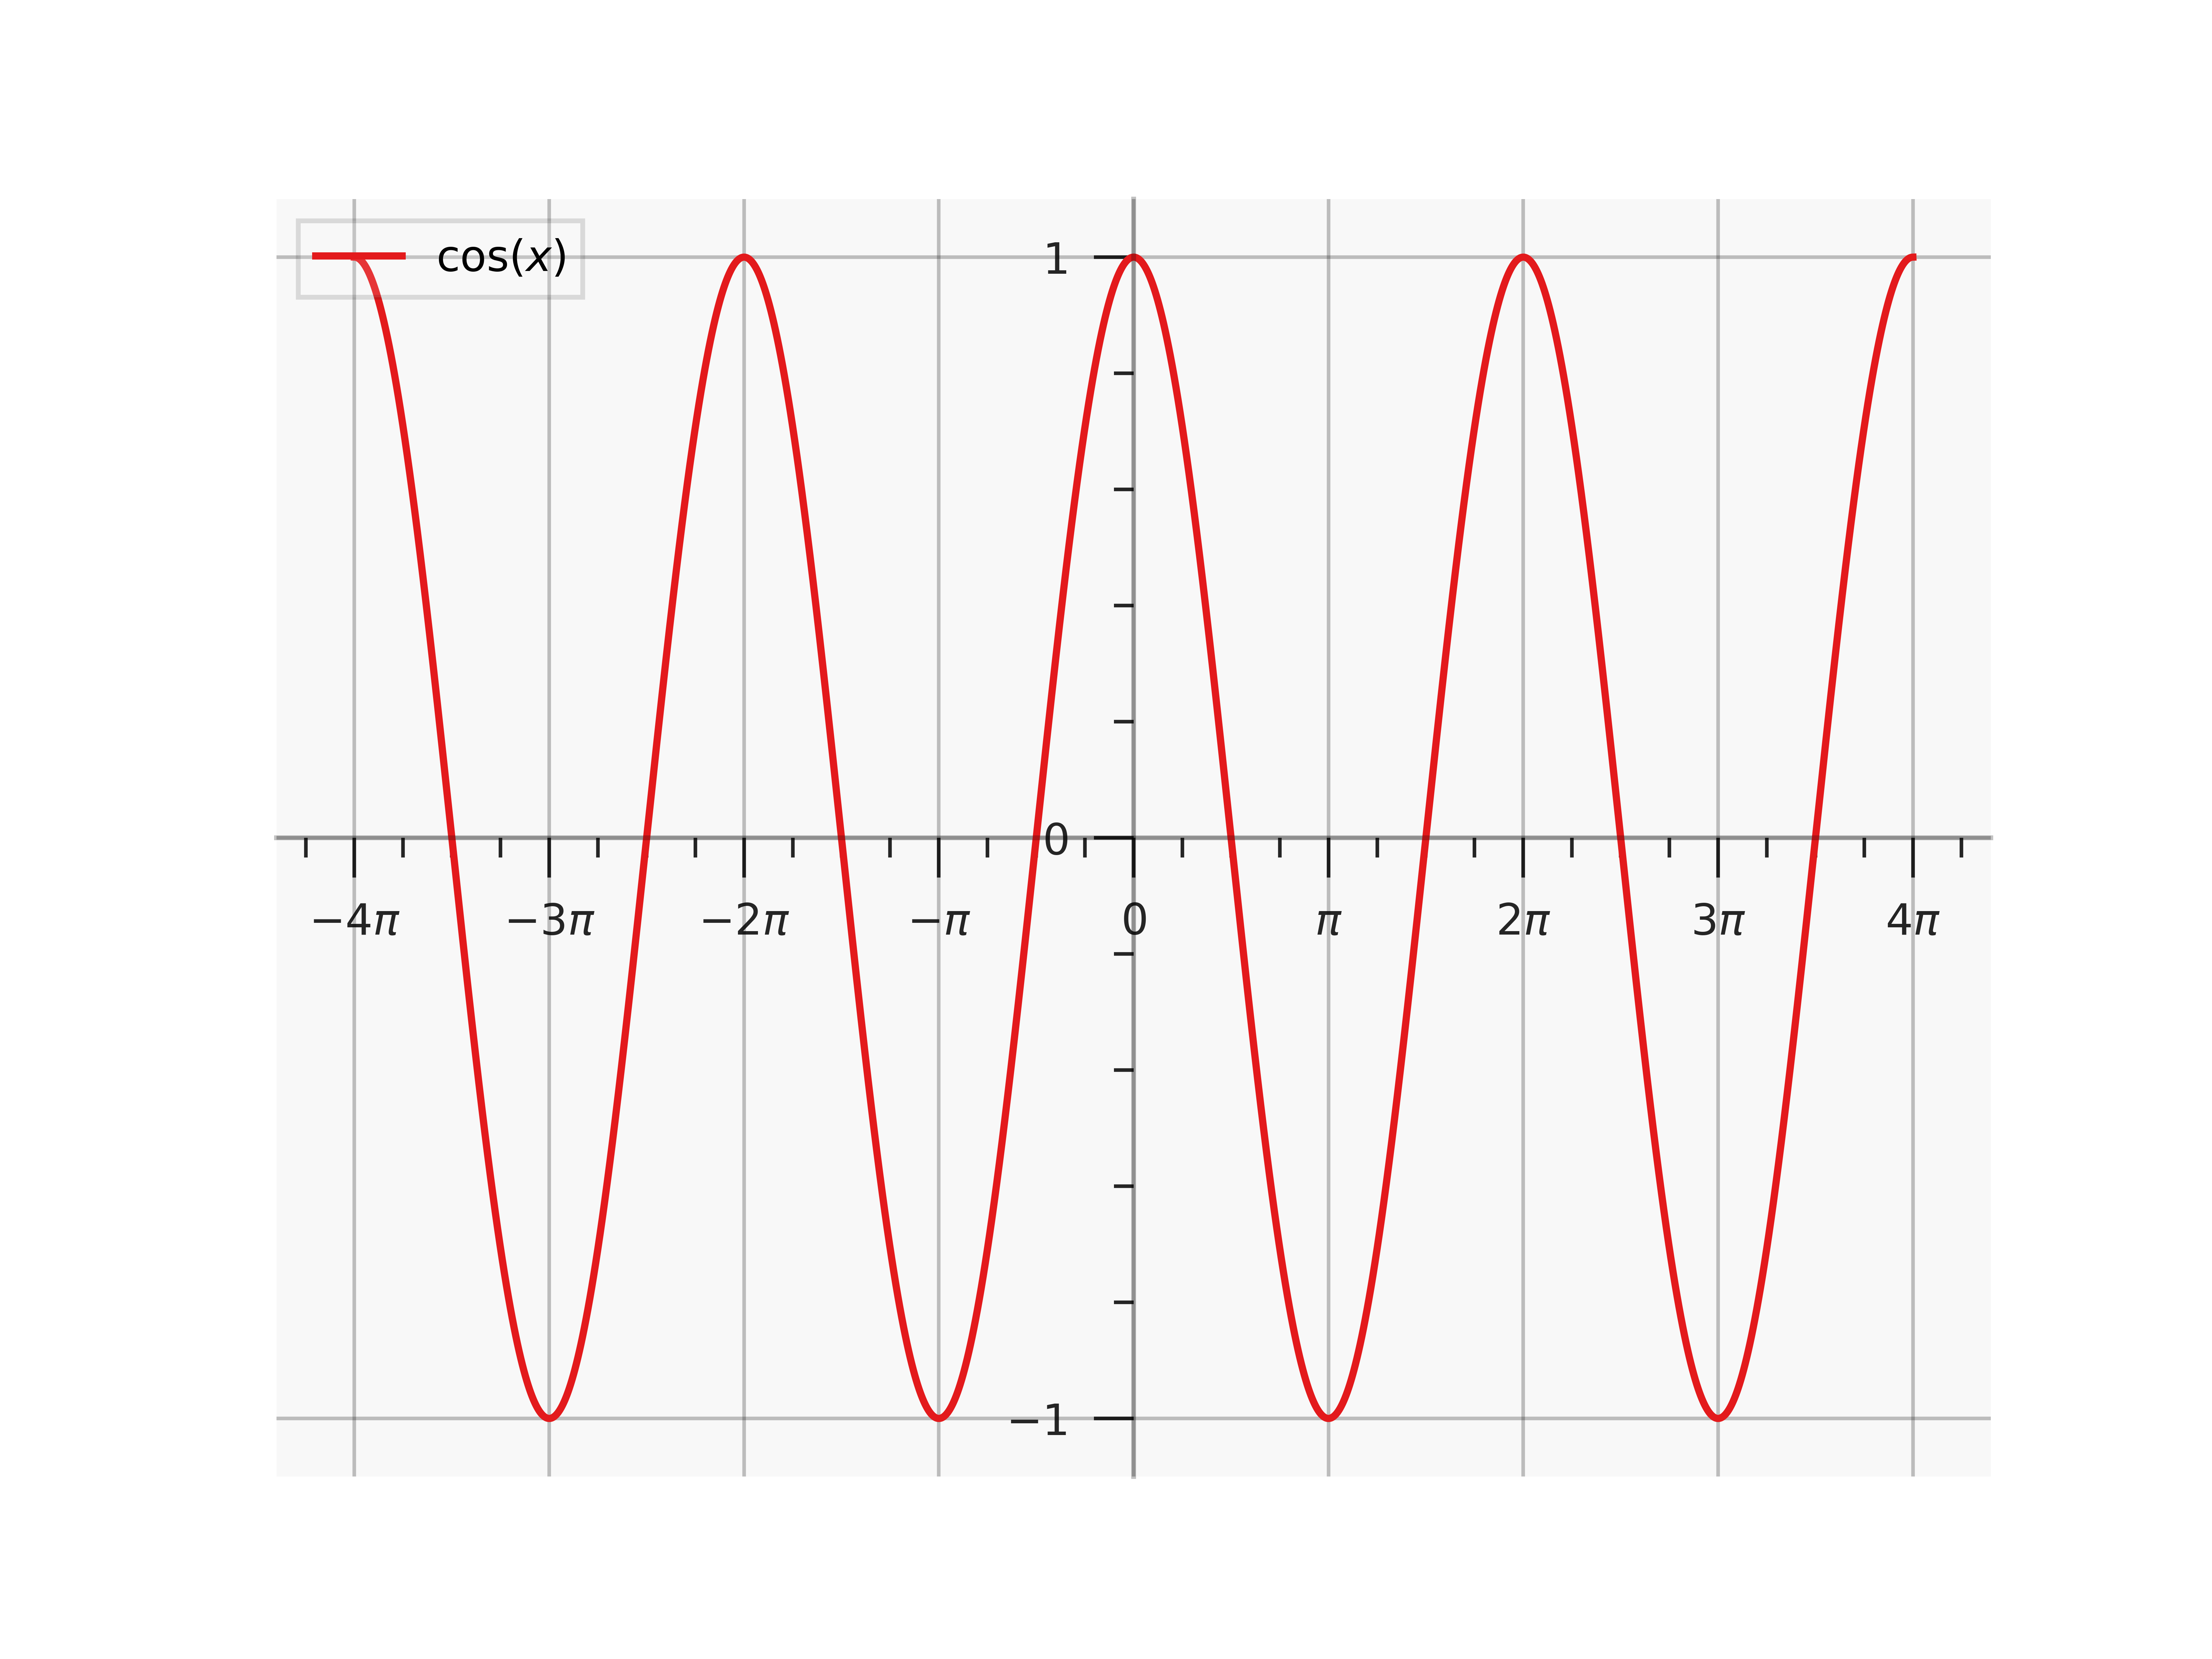
\includegraphics[width=10cm, keepaspectratio]{graph_12.png}
    \caption{Cosine Functions}
    \label{fig:fig12}
\end{figure}

\begin{problem}
Graph $f(x)=\sin(x)$.
\end{problem}

This is quite similar to the cosine function, having the same domain and properties.
The sketch is below.

\begin{figure}[H]
    \centering
    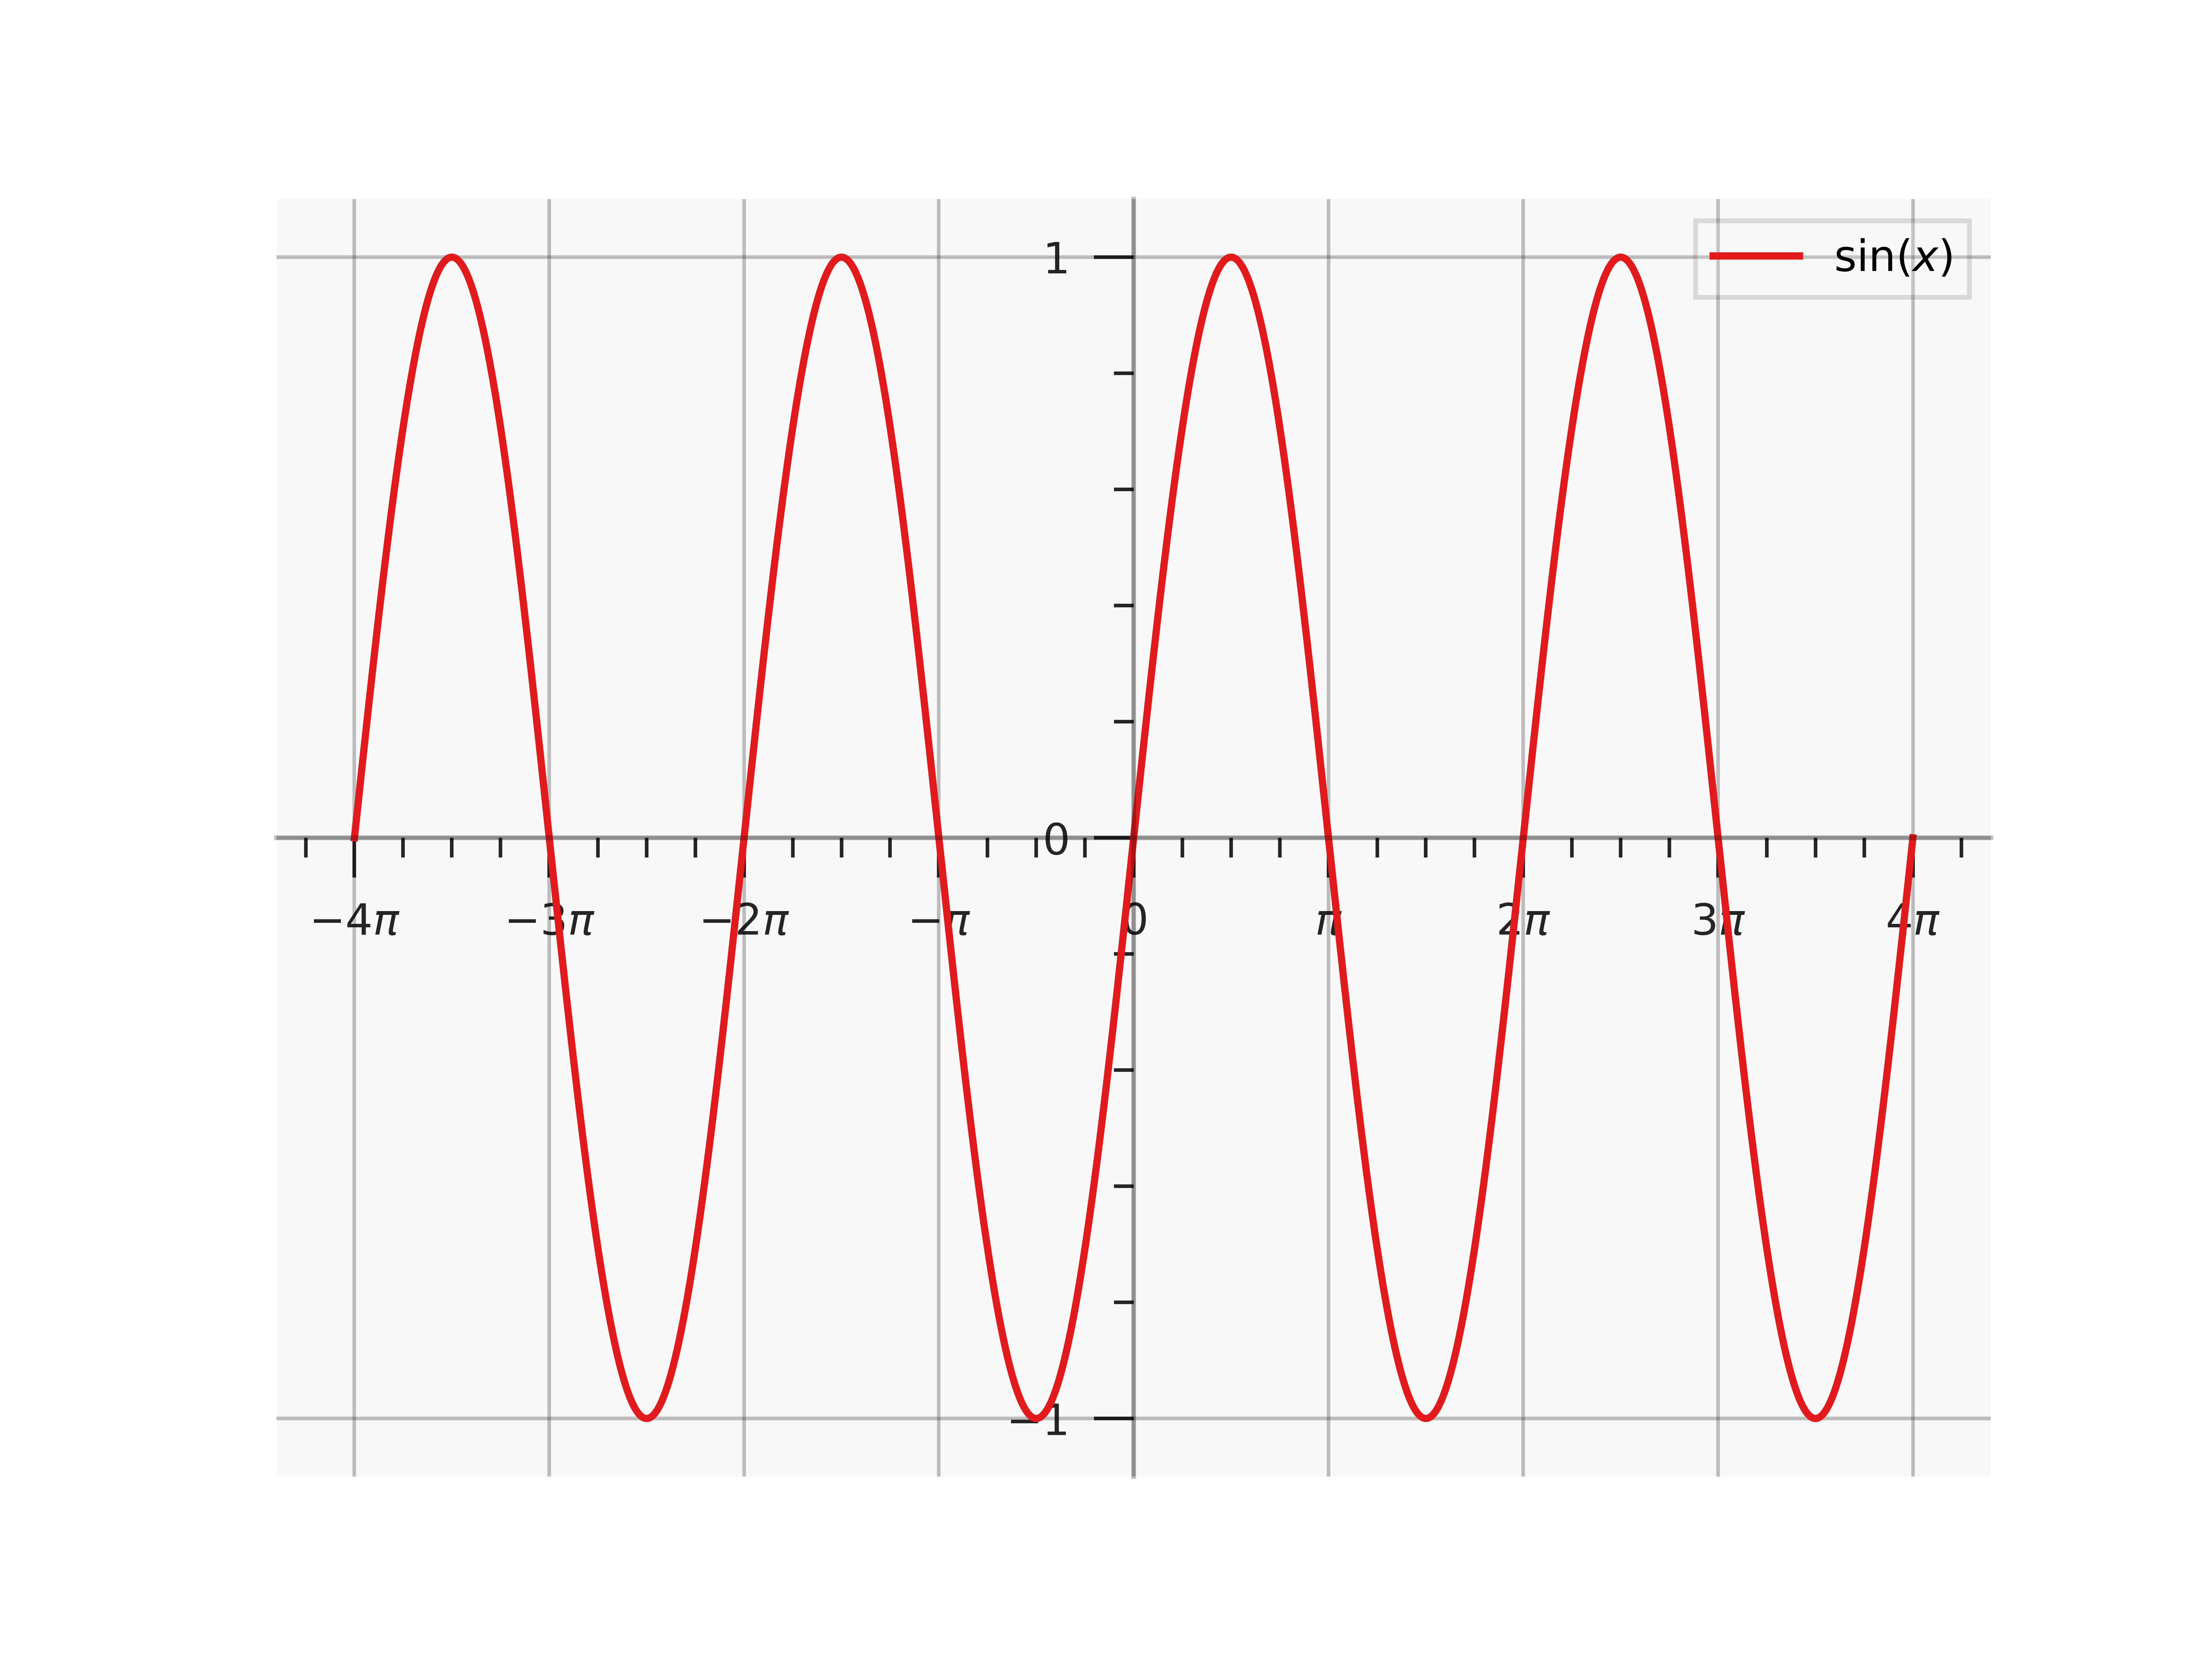
\includegraphics[width=10cm, keepaspectratio]{graph_13.png}
    \caption{Sine Functions}
    \label{fig:fig13}
\end{figure}

\begin{problem}
Graph $f(x)=\tan(x)$.
\end{problem}

The tangent function can be written as $\frac{\sin(x)}{\cos(x)}$.
Therefore, we can see that it will not exist at $x$ values whose cosines are 0.
This means that the tangent function will not exist at:

\begin{equation}
    x \in \left\{\dots, -\frac{5\pi}{2}, -\frac{3\pi}{2}, -\frac{\pi}{2}, \frac{\pi}{2}, \frac{3\pi}{2}, \frac{5\pi}{2}, \dots \right\}
\end{equation}

The graph of tangent will have asymptotes at these points.
Below is the graph of $\tan(x)$ (and its asymptotes) for the interval $-\frac{5\pi}{2} < x < \frac{5\pi}{2}$.

\begin{figure}[H]
    \centering
    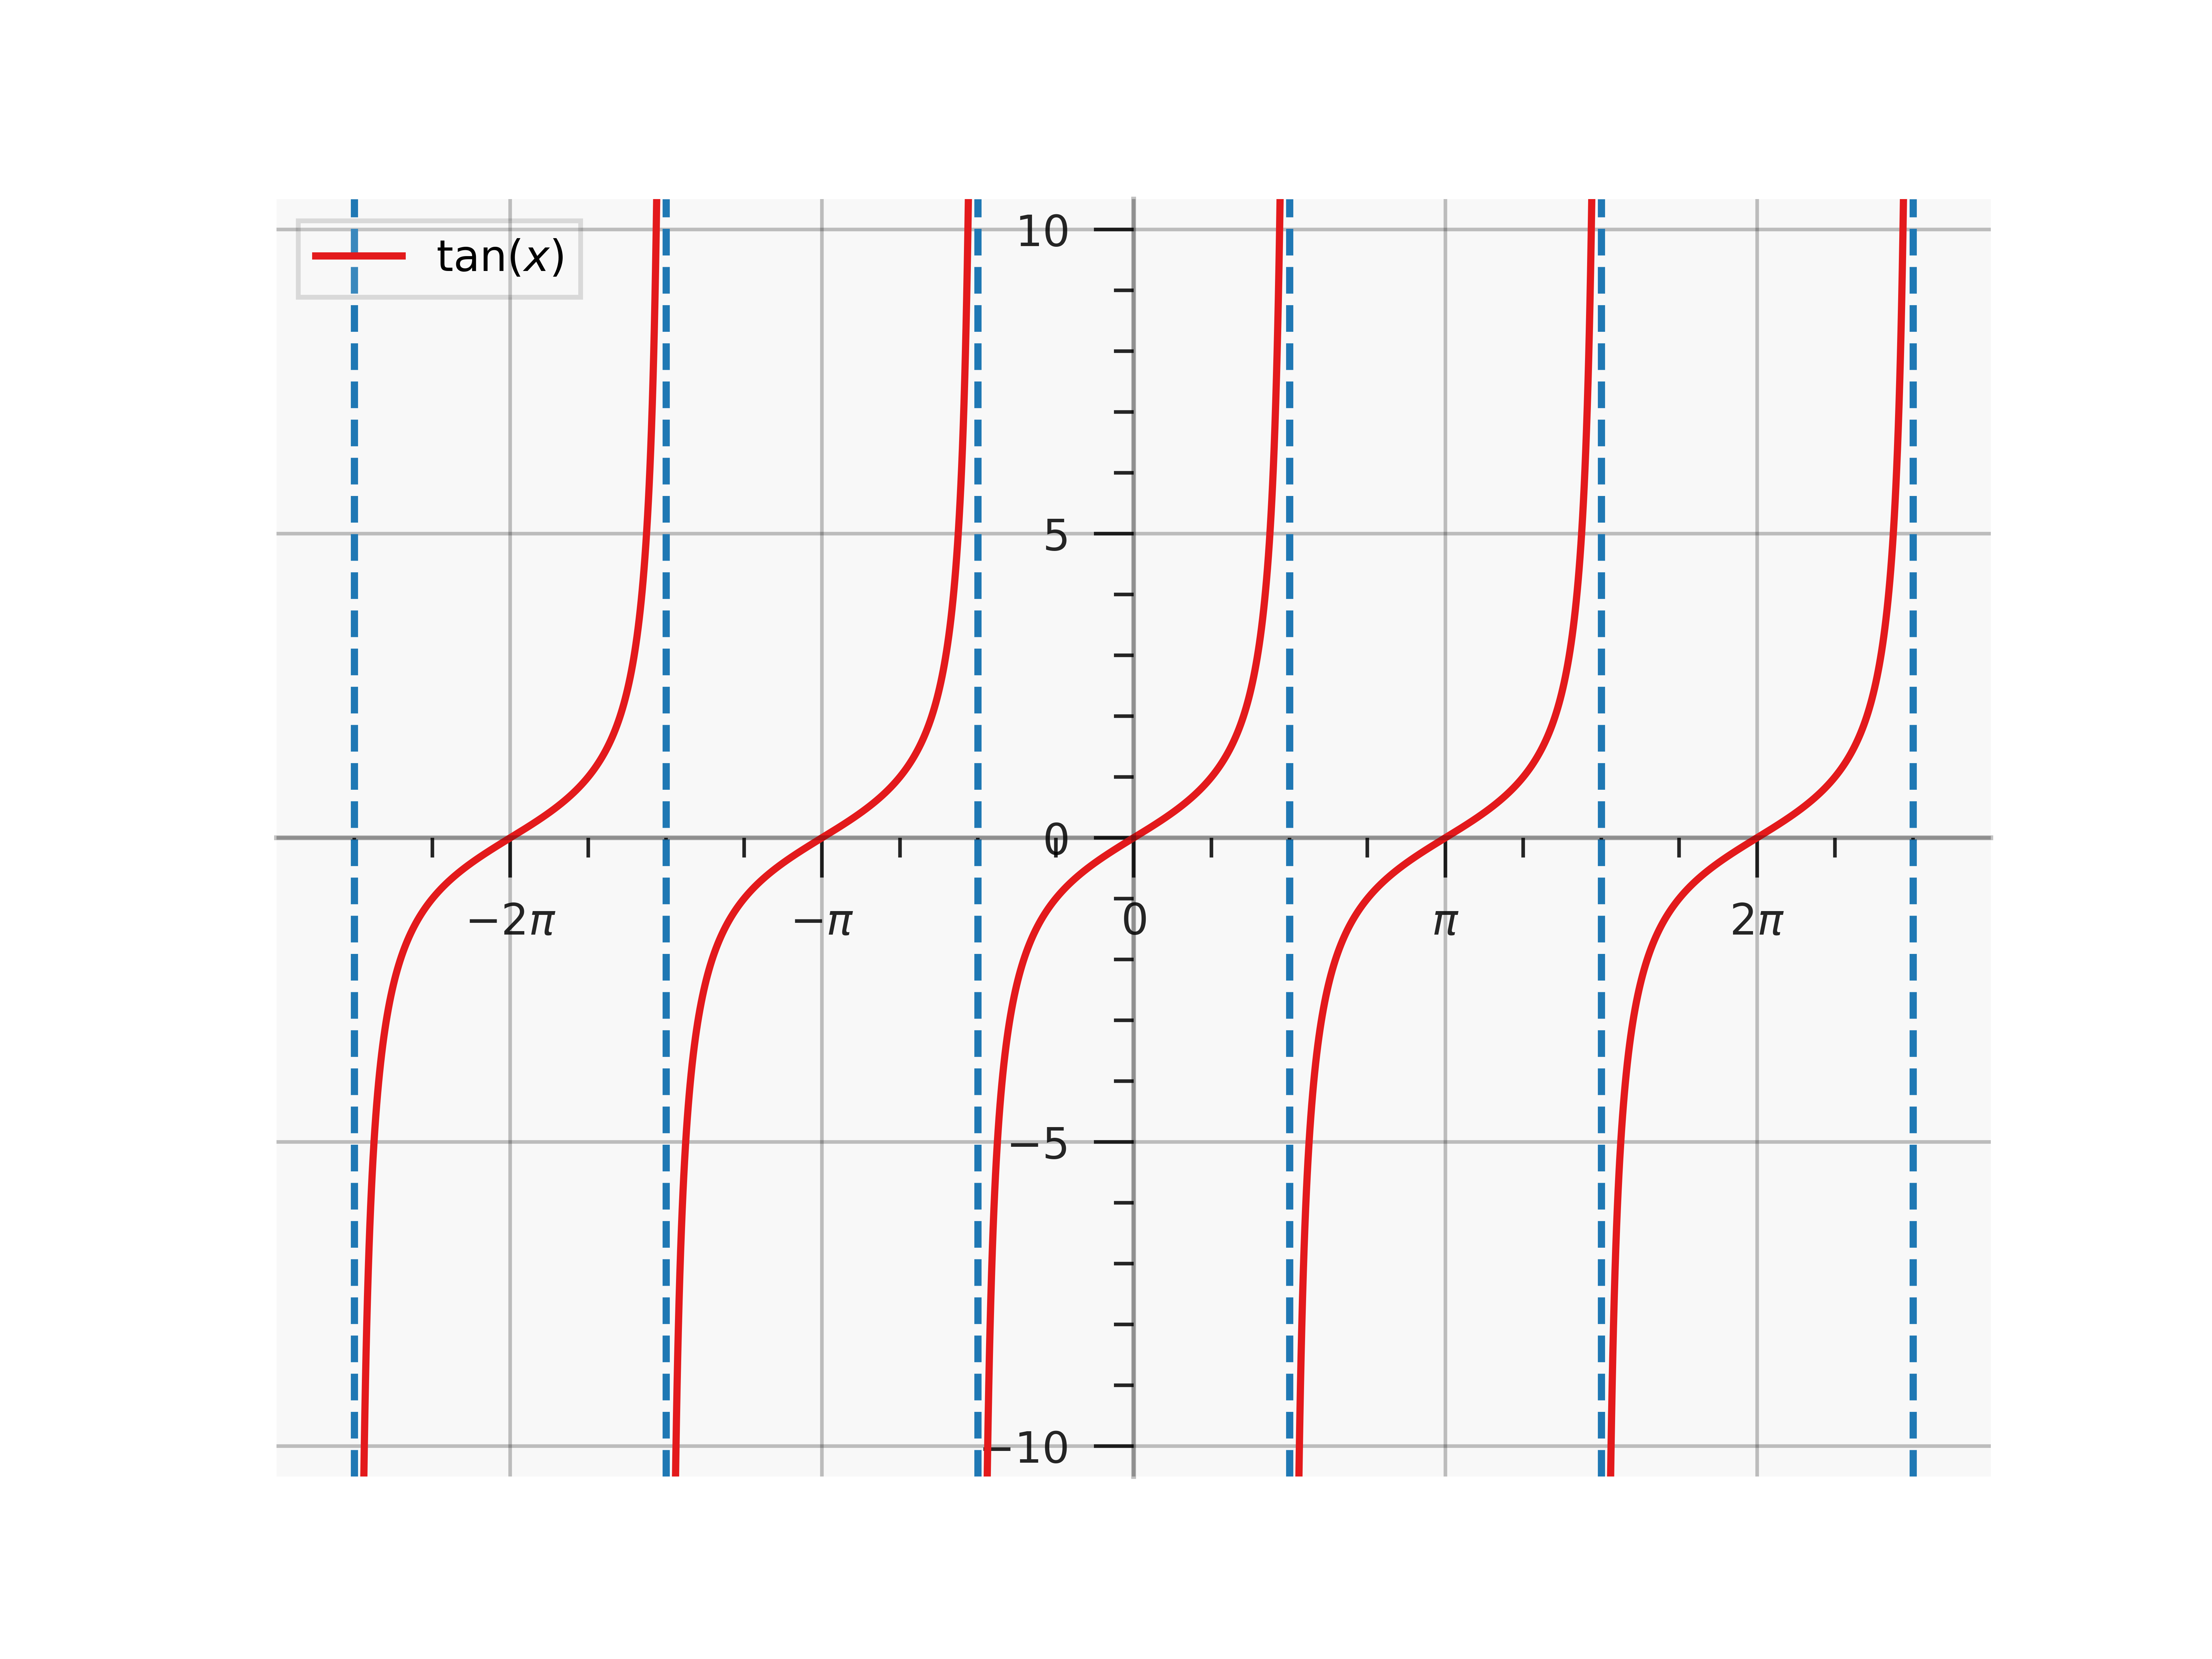
\includegraphics[width=10cm, keepaspectratio]{graph_14.png}
    \caption{Tangent Functions}
    \label{fig:fig14}
\end{figure}

\begin{problem}
Graph $f(x)=\sec(x)$.
\end{problem}

As with the tangent function, the secant function will not exist at points where the cosine function is 0.
This is because it is the reciprocal of the cosine function.
We will find asymptotes at the same points as we did for the tangent function.
Also note that the secant function will always be greater than (or equal to) 1 or less than (or equal to) $-1$.
This is pretty obvious as the inverse is true for the cosine function and the reciprocal of any number between $-1$ and $1$ will give a number outside of that range.
The range for $\sec(\omega x)$ is then $\sec(\omega x) \geq 1$ and $\sec(\omega x) \leq -1$, where $\omega$ is some constant.

The graph of $\sec(x)$ (and its asymptotes) is:

\begin{figure}[H]
    \centering
    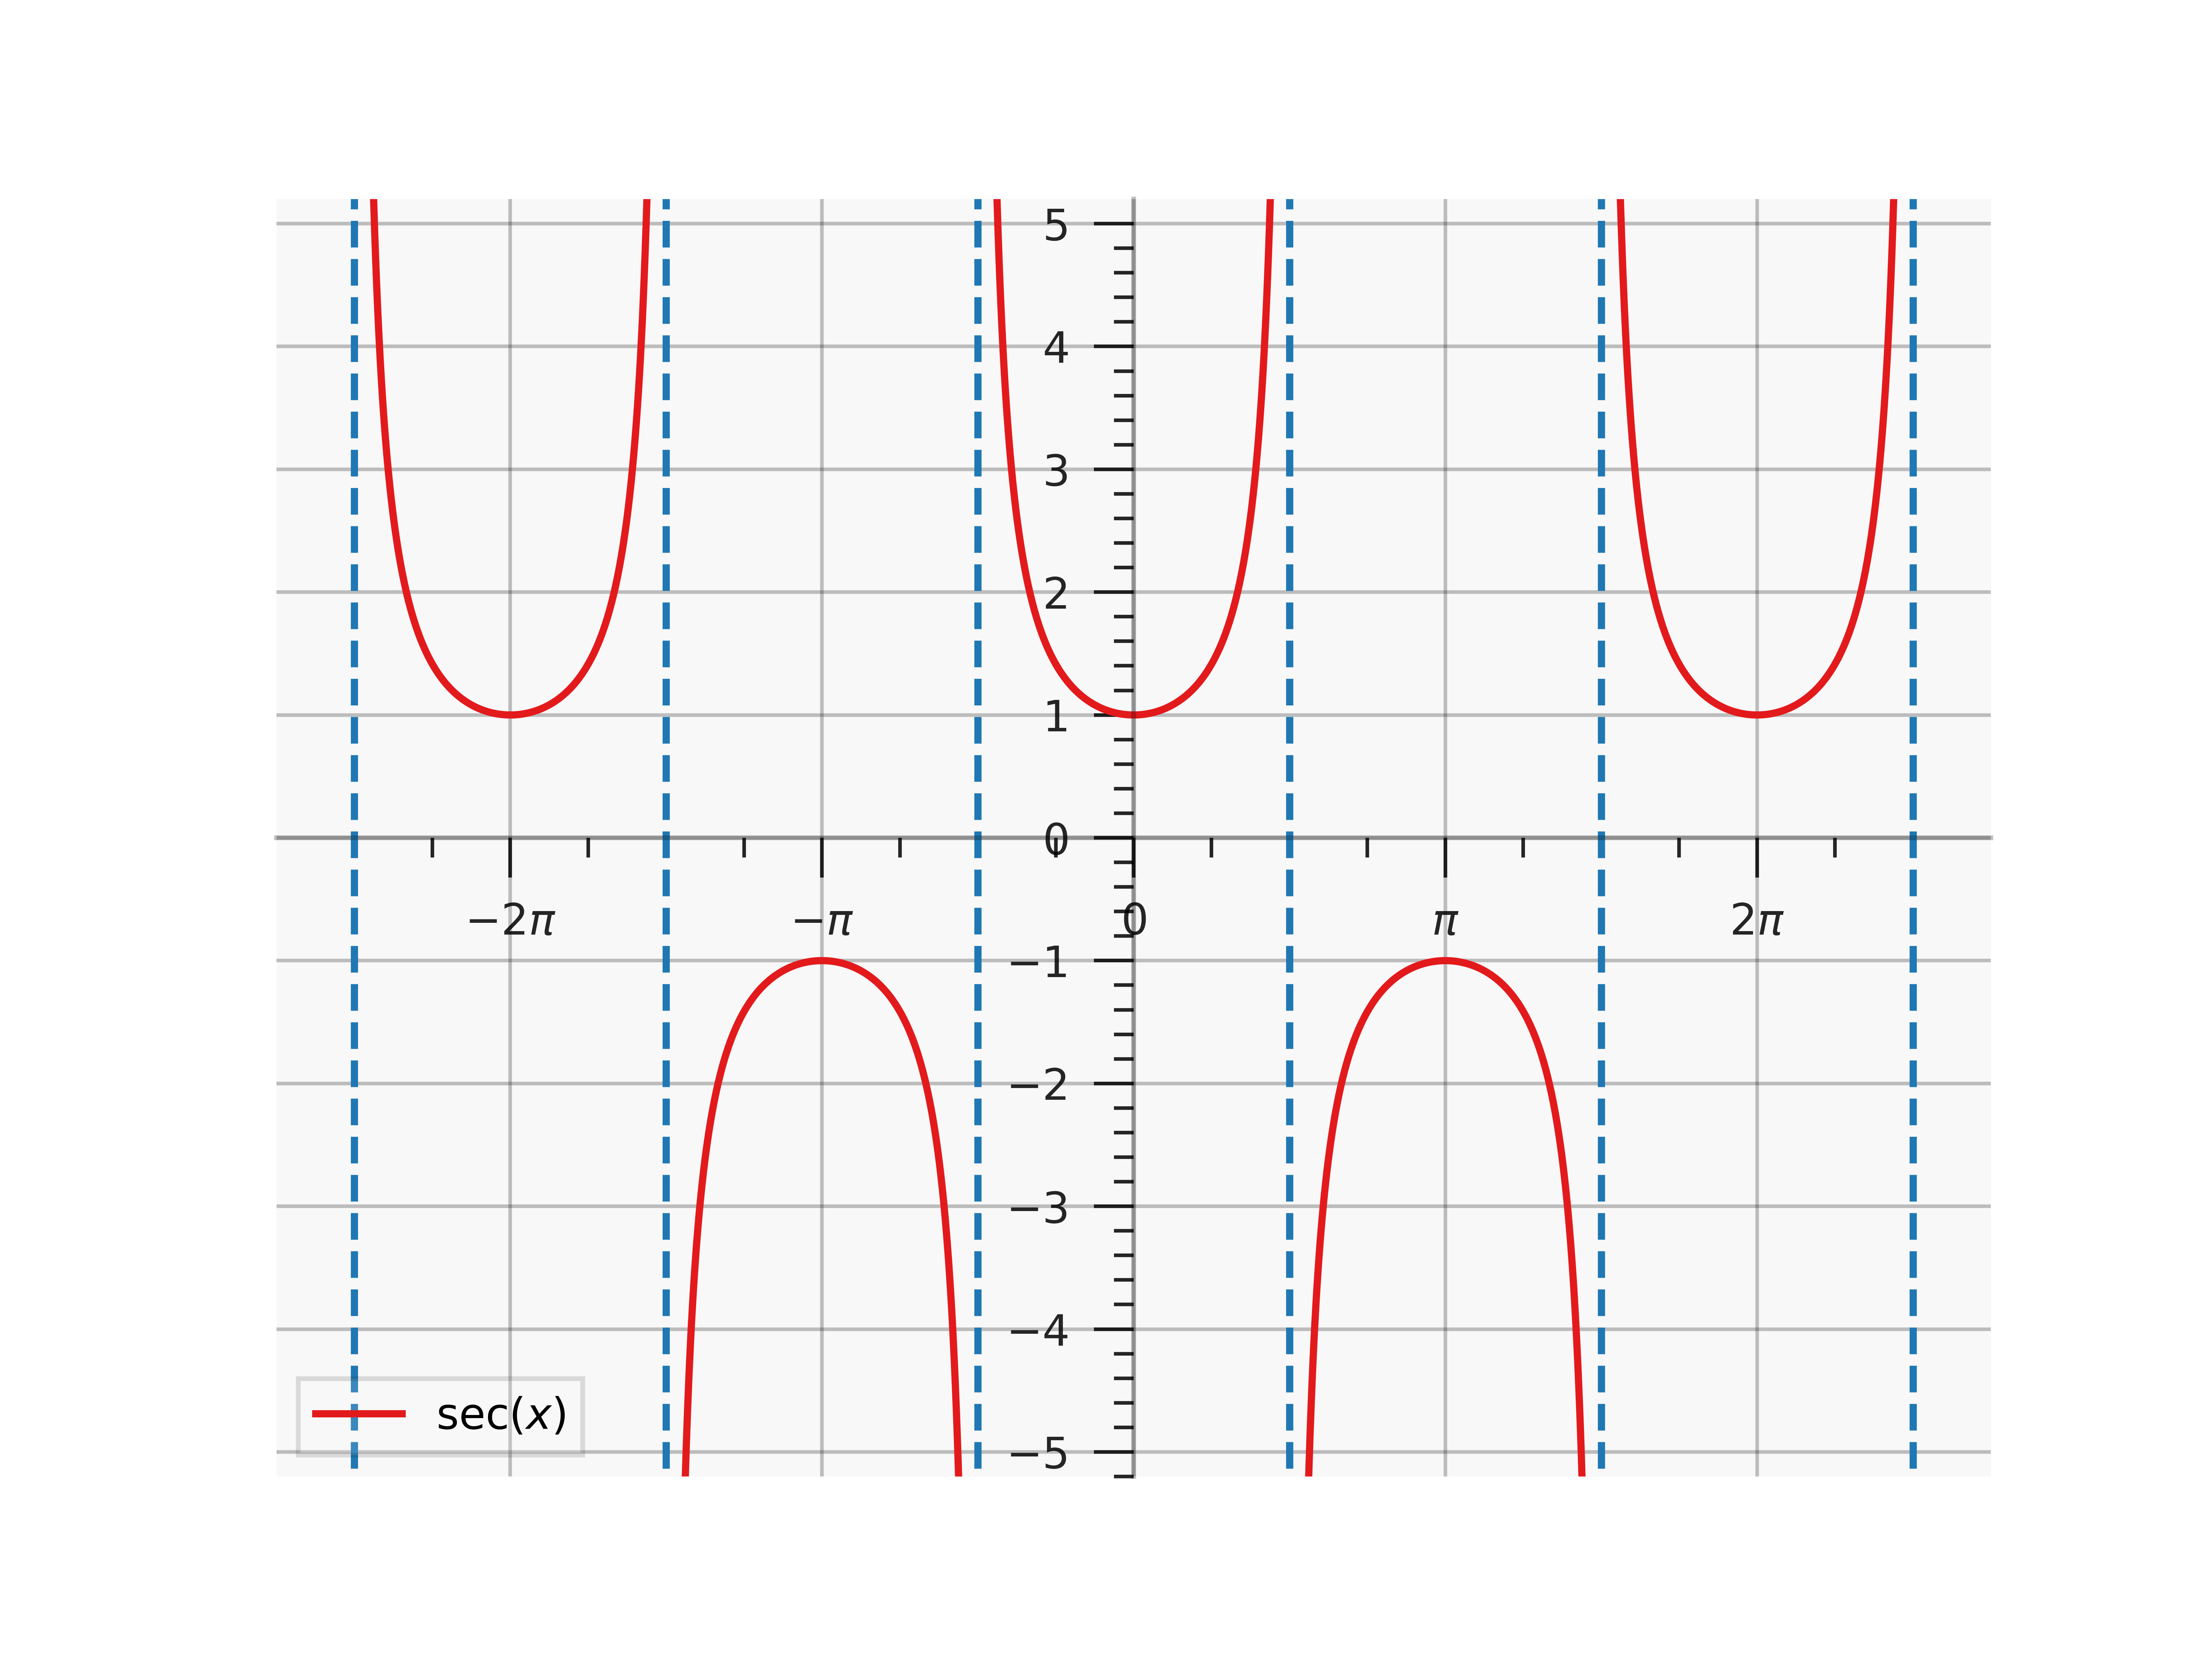
\includegraphics[width=10cm, keepaspectratio]{graph_15.png}
    \caption{Secant Functions}
    \label{fig:fig15}
\end{figure}

Note that the cosecant and cotangent functions were not graphed.
These are quite similar to other trig functions that were graphed however.
Also, transformations of functions were not covered.
Knowing basic transformations can make graphing functions simpler which is helpful in Calculus course.

\end{document}